\documentclass{IEEEtran}
\usepackage{cite}
\usepackage[a4paper, total={7.5in, 10.5in}]{geometry}
\usepackage{multirow}
\usepackage{amssymb}
\usepackage{amsfonts}
\usepackage{algorithmic}
\usepackage{textcomp}
\usepackage{fancyhdr}
\usepackage{titlesec}
\setcounter{secnumdepth}{4}
\usepackage{blindtext}
\usepackage{titlesec}
\usepackage{color}
\usepackage{amsmath}
\usepackage{xcolor}
\usepackage{soul}
\newcommand{\mathcolorbox}[2]{\colorbox{#1}{$\displaystyle #2$}}
\usepackage{authblk}
\usepackage[utf8]{inputenc}
\usepackage{graphicx}
\usepackage{amsmath}
\usepackage[export]{adjustbox}
\usepackage[center]{caption}

\graphicspath{{images/}}

\title{\textbf{Fitting Magic Formula '96 coefficients\\}}

\begin{document}
    \author{\underline{Daniele Vedovelli}}
    \author{\underline{Nicolò Cavalieri}}
    \affil{Department of Industrial Engineering (DII), University of Trento}
   
    \date{A.Y. 2022-2023}
    
    \maketitle
    
    \tableofcontents

    \pagenumbering{arabic}
    
    \bigskip
    \bigskip

    \begin{abstract}
    Tyre models have been developed during the years to satisfy the need of modeling vehicle dynamics. Tyres exhibit non-linear behaviours that require advanced models with many coefficients that shape and fit the curves to data collected from tyre testing machines equipment. The fitted curves are then used to foresee the behaviour of a tyre at any given configuration. This is very important for commercial vehicle dynamics studies, as well as for racing, where the difference between a well modeled tyre and a poor one may lead the team to tune poorly the vehicle. One of the most used models is the Magic Formula '96 (MF96), which can take into account several different effects changing the behaviour of a tyre. The fitting of the MF96 tyre model coefficients on a dataset of measured tyre forces for a  F-SAE tyre was required as the first assignment of Dynamics of Vehicles course held by Professor F.Biral. Many different subsequent steps will be presented in the following pages together with comments and plots.
    \end{abstract}
    
    \section{\textbf{Introduction}}
     The scope of this first assignment was to fit the MF96 tyre model to Formula SAE tyre data collected by Calspan Tire Research Facility (TIRF) during the Round 5 testing. The provided datasets contained data for the following tyres:
        \begin{itemize}
                \item Continental 205 / 510 R13 (C11/C12)
                \item Goodyear D2704 20.0x7.0-13
                \item Hoosier 18.0 x 6.0 - 10 R25B
        \end{itemize}

    Each dataset was composed by two \texttt{.mat} files:
      \begin{enumerate}
            \item the first for the identification of the pure longitudinal and combined forces;
            \item the second for the identification of the pure lateral force and the self aligning moment.\\
        \end{enumerate} 

        The fitting discussed in these pages is to be referred to Hoosier tyres and the obtained coefficients are for MF96 in ISO reference frame (Fig.~\ref{fig:ISO}).
        
     
        \begin{figure}[htbp]
            \centerline{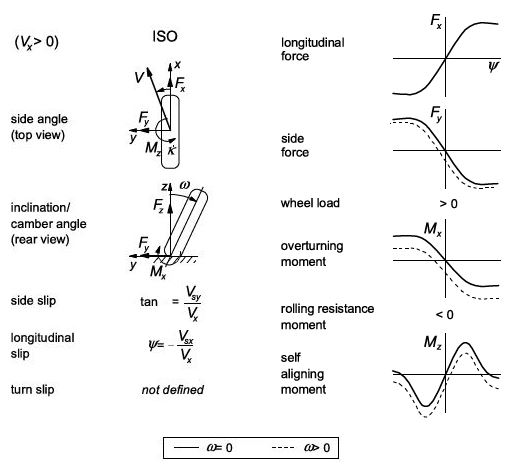
\includegraphics[width= \columnwidth]{ISO.JPG}}
            \caption{\textbf{ISO reference frame for MF96 formula}
            \text{(Credits: Tyre and vehicle dynamics, Hans B. Pacejka)}}
            \label{fig:ISO}
        \end{figure}
    
        \newpage
    
    \section{\textbf{MF96 coefficients tyre data fitting procedure}}
        Fitting has been carried out in \textsc{Matlab}$^{\circledR}$ using a least-squares approach, as suggested, and \texttt{fmincon} as the non linear optimization solver. Parameters, as initial guesses and upper and lower bounds for \texttt{fmincon}, fitted coefficients values, $R^{2}$ and $RMSE$ are reported for each fitting procedure carried out in the developed script.

        Sample ranges used for fitting were the following:
        \begin{itemize}
            \item $\texttt{Hoosier\_B1464run23.mat} \rightarrow 27760:54500$
            \item $\texttt{Hoosier\_B1464run30.mat} \rightarrow 19028:37643$\\
        \end{itemize}
        
        \newpage
    
    \subsection{\textbf{\underline{Pure longitudinal force}}}
        Fitting of the pure longitudinal force $F_{x_0}$ coefficients with the following 3 steps:
        \begin{itemize}
            \item Fitting of coefficients with \textbf{pure conditions: nominal vertical load $F_{z_0} = 220 \, [N]$ and zero camber angle $\gamma = 0 \, [deg]$ }\\
        
                \begin{table}[htpb]
                \begin{adjustbox}{width=\columnwidth,center}
                  
                    \begin{tabular}{|l|l|l|l|l|l|l|l|}
                    \hline
                    Coefficients       & $pC{x_1}$   & $pD_{x_1}$   & $pE_{x_1}$   & $pE_{x_4}$   & $pK_{x_1}$    & $pH_{x_1}$        & $pV_{x_1}$    \\ \hline
                    $P_0$ - initial guess & 1      & 2      & 1      & 0      & 0       & 1           & 0       \\ \hline
                    lb - lower bound   & 1      & 0.1    & 0      & 0      & -10     & 0           & -10     \\ \hline
                    ub - upper bound   & 2      & 4      & 1      & 1      & 10      & 100         & 10      \\ \hline
                    Fitted value       & 1.5387 & 3.1469 & 0.0113 & 0.0806 & 82.4171 & -2.0920e-05 & -0.0858 \\ \hline
                    \end{tabular}
                    
                    \end{adjustbox}
                \end{table}
    
                
                \begin{figure}[htbp]
                    \centerline{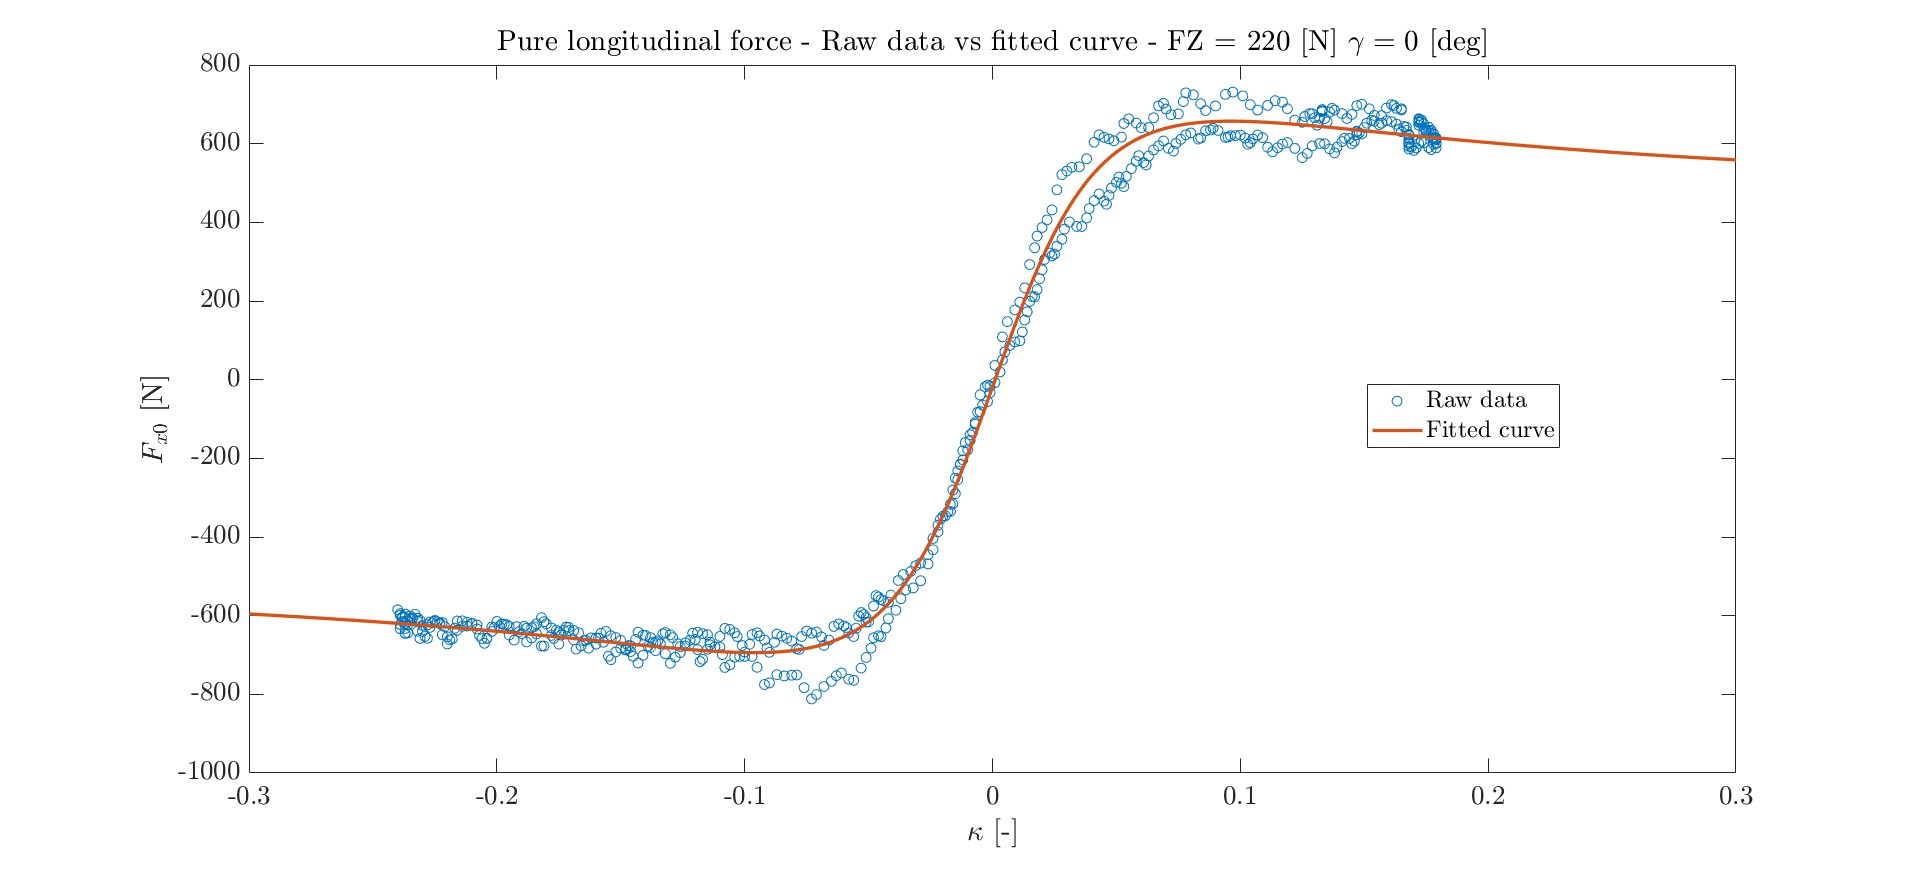
\includegraphics[width = 3.95in]{pure_longitudinal_1.jpg}}
                    
                    \label{fig:nominal conditions Fx0}
                \end{figure}
                
              
                
                \textbf{\textcolor{blue}{Obtained performance indexes}}: \\ $R^{2} = 99.55 \, \%$ and $RMSE = 40.47 \, $ \, [N] .\\\\
                

            \item Fitting of coefficients depending on \underline{$df_z$} \textbf{load variation with zero camber angle $\gamma = 0$}
                \begin{table}[!h]
                \begin{adjustbox}{width=\columnwidth,center}
                    
                    \begin{tabular}{|l|l|l|l|l|l|l|l|}
                    \hline
                    Coefficients       & $pD_{x_2}$    & $pE_{x_2}$    & $pE_{x_3}$   & $pH_{x_2}$  & $pK_{x_2}$    & $pK_{x_3}$   & $pV_{x_2}$    \\ 
                    \hline
                    $P_0$ - initial guess & 0       & 0       & 0      & 0      & 0       & 0      & 0       \\ \hline
                    lb - lower bound   & -       & -       & -      & -      & -       & -      & -       \\ \hline
                    ub - upper bound   & -       & -       & -      & -      & -       & -      & -       \\ \hline
                    Fitted value       & -0.2496 & -0.3619 & 0.1059 & 0.0011 & -0.0019 & 0.1536 & -0.0256 \\ \hline
                    \end{tabular}
                    \end{adjustbox}
                \end{table}
                
                
                \begin{figure}[!h]
                    \centerline{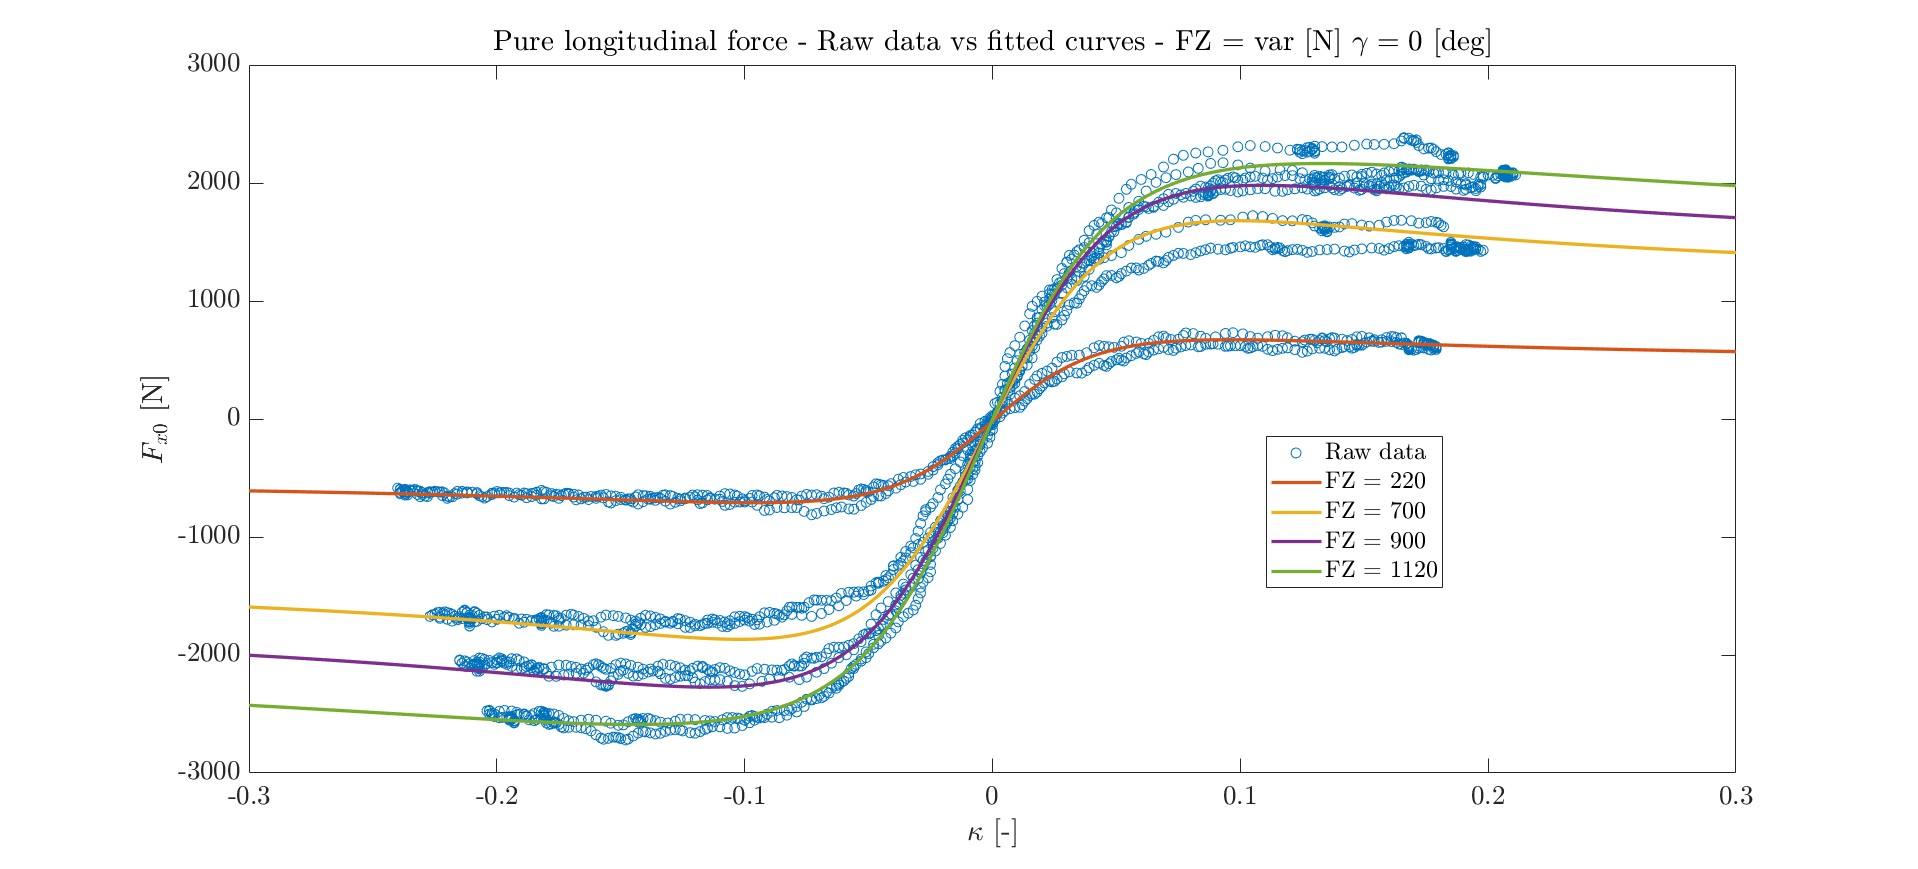
\includegraphics[width = 3.95in]{pure_longitudinal_2.jpg}}
                   
                    \label{fig:variable load Fx0}
                \end{figure}
                \textbf{\textcolor{blue}{Obtained performance indexes}}: \\ $R^{2} = 99.71 \, \%$ and $RMSE = 85.91 $ \, [N] .\\\\
            \newpage
                
                               
            \item Fitting of coefficients depending on \textbf{variable camber $\gamma$ and nominal vertical load $F_{z_0} = 220$ [N]}
            \begin{table}[htbp]
                \begin{center}
                \begin{tabular}{|l|l|}
                \hline
                Coefficients       & $pD_{x_3}$    \\ \hline
                $P_0$ - initial guess & 0       \\ \hline
                lb - lower bound   & -       \\ \hline
                ub - upper bound   & -       \\ \hline
                Fitted value       & 18.4364 \\ \hline
                \end{tabular}
                \end{center}
            \end{table}
            
        
                \begin{figure}[htbp]
                    \centerline{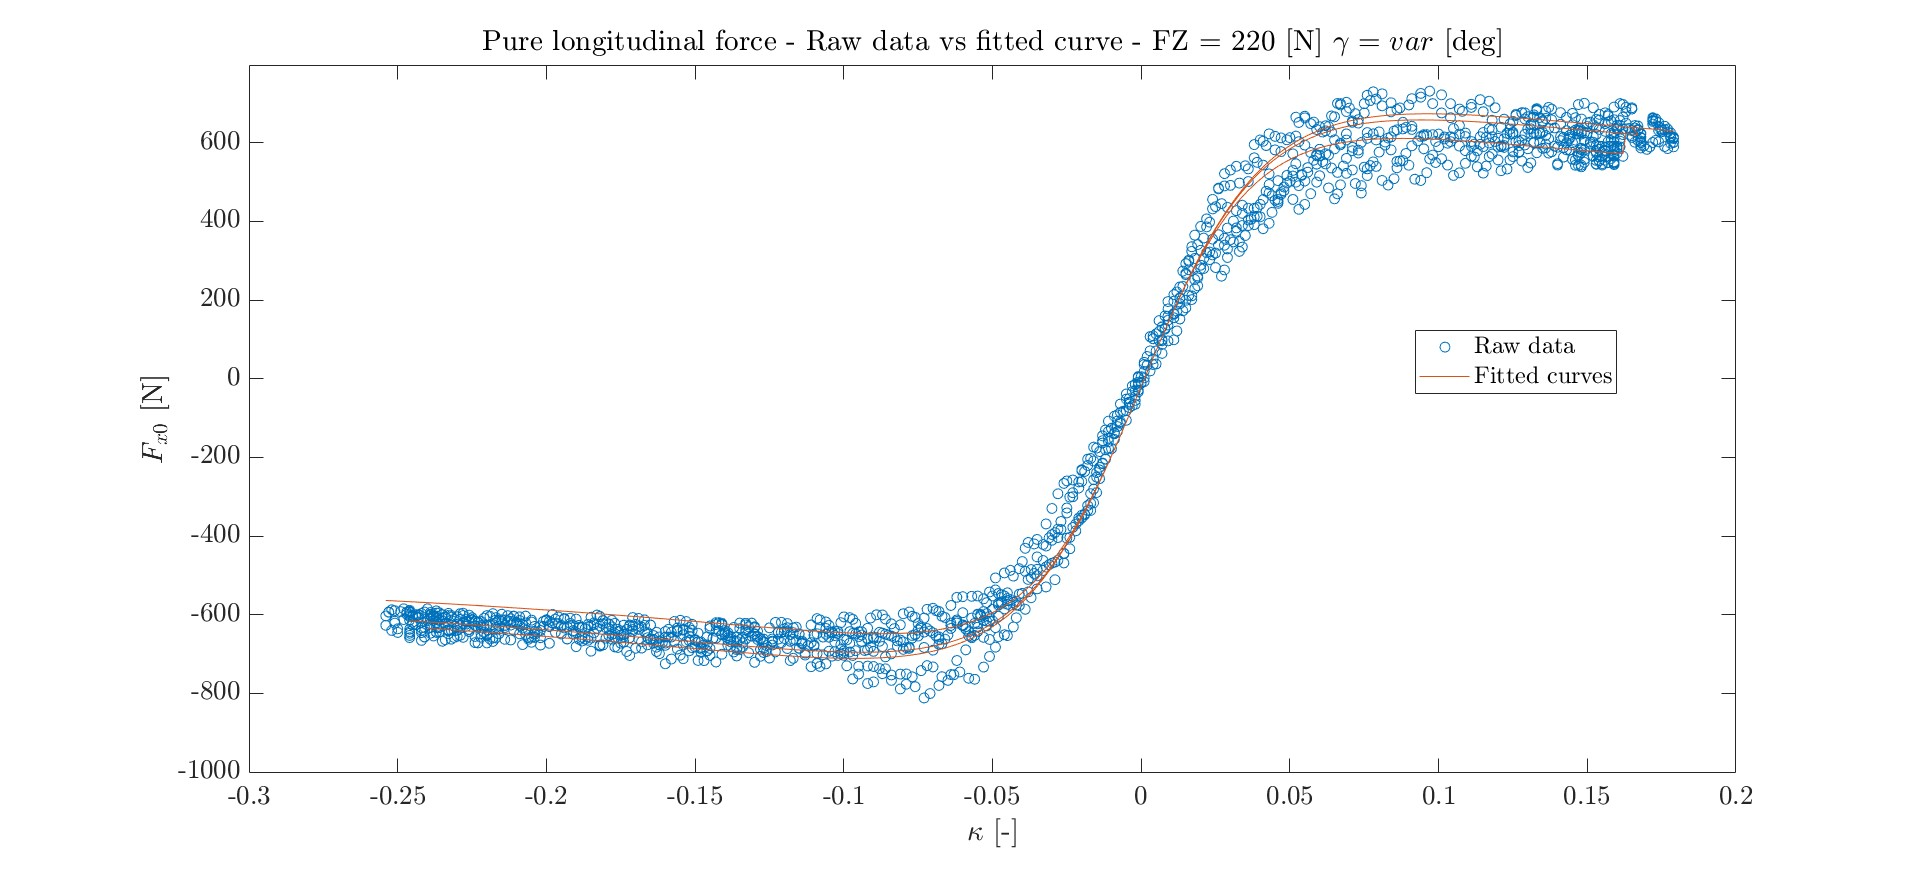
\includegraphics[width = 3.95in]{pure_longitudinal_3.jpg}}
                   
                    \label{fig:variable camber Fx0}
                \end{figure}
            
            
          
            \textbf{\textcolor{blue}{Obtained performance indexes}}: \\ $R^{2} = 99.03 \, \%$ and $RMSE = 57.45 $ \, [N] . \\\\

            The longitudinal slip stiffness is plotted as shown below 

            \centerline{}
                \begin{figure}[htbp]
                    \centerline{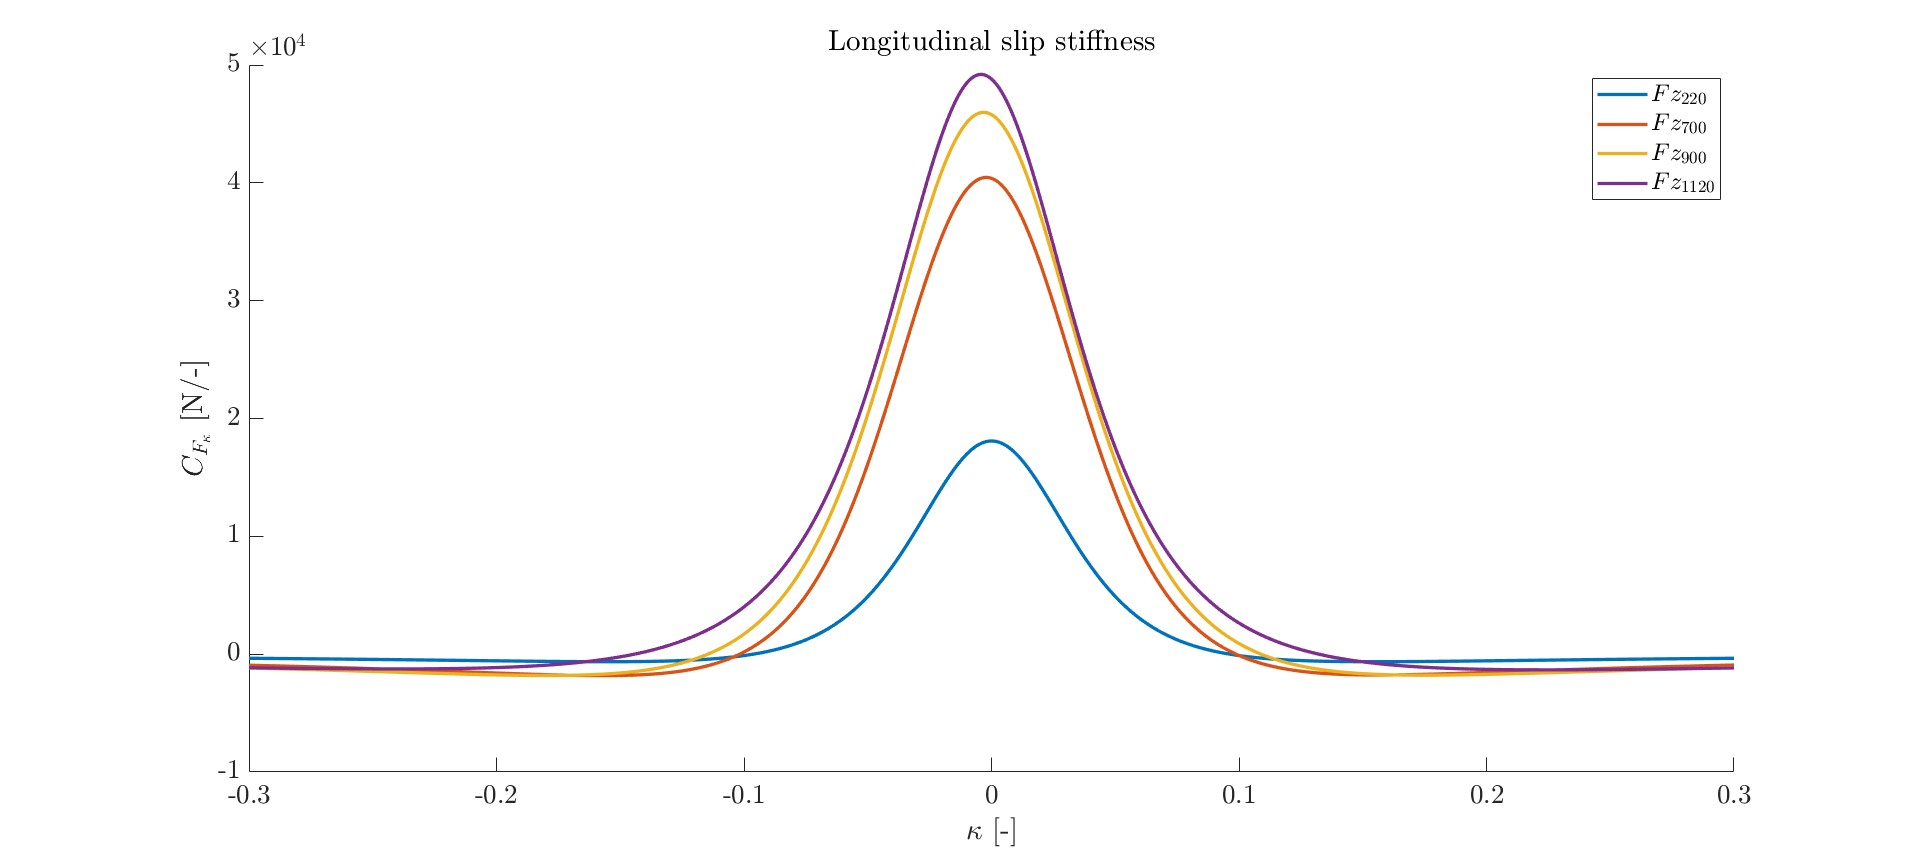
\includegraphics[width = 3.95in]{longitudinalK.jpg}}
                    
                    \label{fig:LongStiff}
                \end{figure}
            
        \end{itemize}
        
        \textit{\underline{COMMENTS}}: It can be observed that, for some vertical load cases, the current fitting overestimates or underestimates the longitudinal force for certain values of the slip ratio $\kappa$. This may introduce some inaccuracies when using the MF96 curves to predict the behaviour of the tyre. A finer tuning of the coefficients may solve these problems. 

        \newpage
        
    \subsection{\textbf{\underline{Pure lateral force}}}
        Fitting of the pure lateral force $F_{y_0}$ coefficients with the following 4 steps:
        \begin{itemize}
            \item Fitting of coefficients with \textbf{pure conditions: vertical nominal load $F_{Z_0} = 1120$ [N] and zero camber angle $\gamma = 0$ [deg]} \\
        
                \begin{table}[htbp]
                \begin{adjustbox}{width=\columnwidth,center}
                    \begin{tabular}{|l|l|l|l|l|l|l|l|}
                    \hline
                    Coefficients       & $pC_{y_1}$   & $pD_{y_1}$   & $pE_{y_1}$   & $pH_{y_1}$    & $pK_{y_1}$     & $pK_{y_2}$   & $pV_{y_1}$    \\ \hline
                    $P_0$ - initial guess & 0.1    & 0.1    & 0.1    & 0.1     & 0.1      & 0.1    & 0.1     \\ \hline
                    lb - lower bound   & 1      & -1000  & -1000  & -1000   & -1000    & -1000  & -1000   \\ \hline
                    ub - upper bound   & 2      & 1000   & 1000   & 1000    & 1000     & 1000   & 1000    \\ \hline
                    Fitted value       & 1.0177 & 3.7104 & 1.4733 & -0.0046 & -23.1279 & 1.1343 & -0.0357 \\ \hline
                    \end{tabular}
                    \end{adjustbox}
                \end{table}
    
               
                \begin{figure}[htbp]
                    \centerline{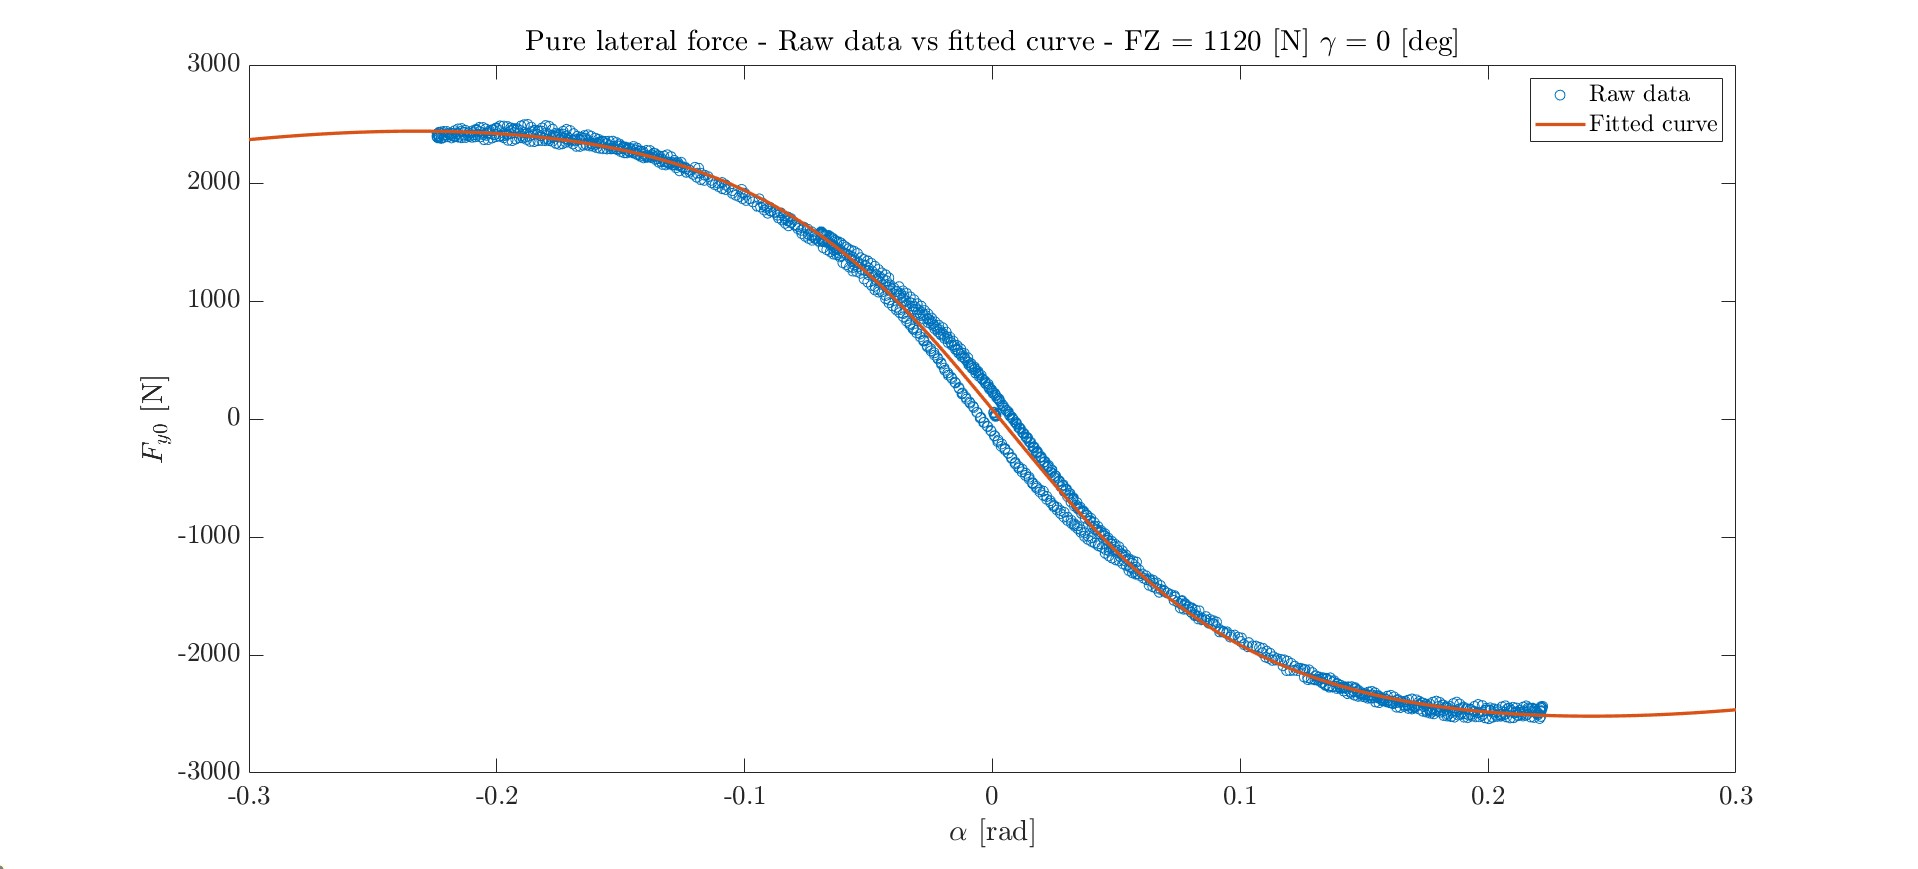
\includegraphics[width = 3.95in]{pure_lateral_1.jpg}}
                   
                    \label{fig:Fy0nom}
                \end{figure}

                \textbf{\textcolor{blue}{Obtained performance indexes}}: \\ $R^{2} = 99.82 \, \%$ and $RMSE = 68.62 \, $[N] .\\\\
                
            \item Fitting of coefficients depending on \underline{$df_z$} \textbf{load variation with zero camber angle $\gamma = 0$}
                \begin{table}[htbp]
                \begin{center}
                    \begin{tabular}{|l|l|l|l|l|}
                    \hline
                    Coefficients       & $pD_{y_2}$    & $pE_{y_2}$       & $pH_{y_2}$        & $pV_{y_2}$   \\ \hline
                    $P_0$ - initial guess & 0.1     & 0.1        & 0.1         & 0.1    \\ \hline
                    lb - lower bound   & -1000   & 0          & -1000       & -1000  \\ \hline
                    ub - upper bound   & 1000    & 1          & 1000        & 1000   \\ \hline
                    Fitted value       & -1.3805 & 8.4470e-05 & -2.8188e-04 & 0.0310 \\ \hline
                    \end{tabular}
                    \end{center}
                \end{table}
                
                
                \begin{figure}[htbp]
                    \centerline{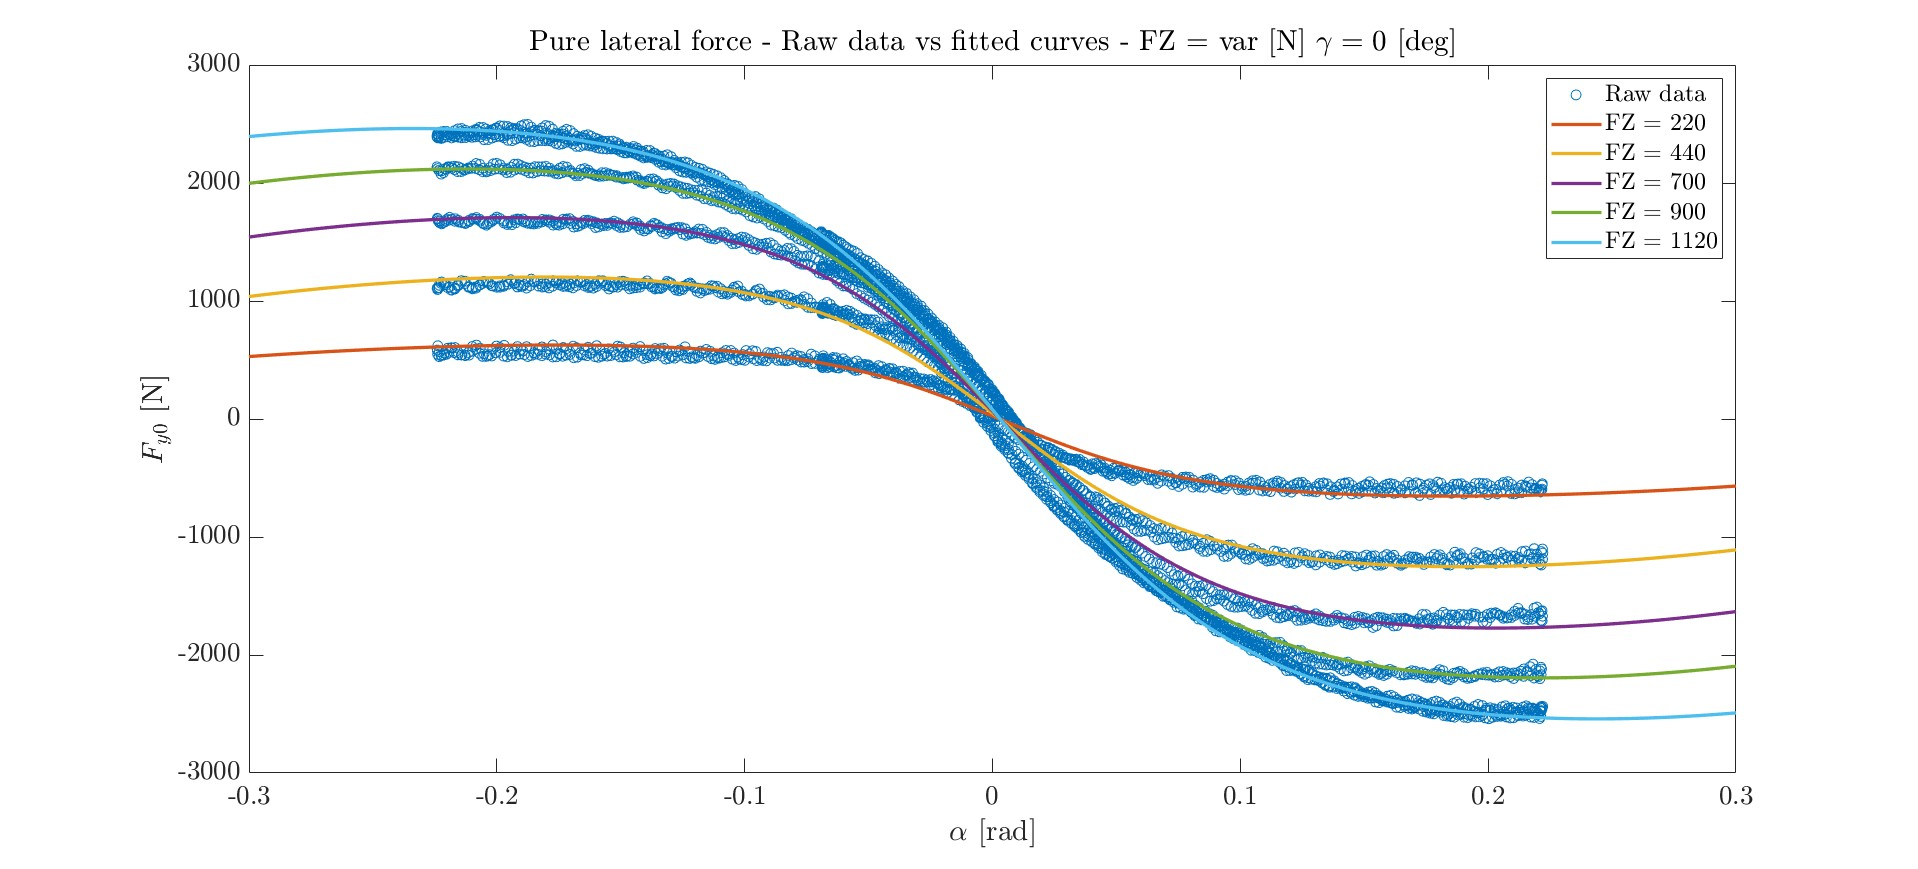
\includegraphics[width = 3.95in]{pure_lateral_2.jpg}}
                    
                    \label{fig:Fy0dfz}
                \end{figure}
    
            

            \textbf{\textcolor{blue}{Obtained performance indexes}}: \\ $R^{2} = 99.68 \, \%$ and $RMSE = 75.19 $ \, [N] .
            \newpage
            \item Fitting of coefficients depending \textbf{on variable camber $\gamma$ and vertical nominal load $F_{Z_0} = 1120$ [N]}
            
                \begin{table}[htbp]
                \begin{adjustbox}{width=\columnwidth,center}
                    \begin{tabular}{|l|l|l|l|l|l|l|}
                    \hline
                    Coefficients       & $pD_{y_3}$    & $pE_{y_3}$       & $pE_{y_4}$        & $pH_{y_3}$ & $pK_{y_3}$ & $pV_{y_3}$    \\
                    \hline
                    $P_0$ - initial guess & 0.1  & 0.5        & 0.1         & 0.1 & 0.1 & 5   \\ \hline
                    lb - lower bound   & -   & -          & -       & - & - & -  \\ \hline
                    ub - upper bound   & -    & -          & -        & - & - & -   \\ \hline
                    Fitted value       & 3.0508 & 0.0077 & -4.0472 & -0.2662 & 0.9497 & -1.7757 \\ \hline
                    \end{tabular}
                    \end{adjustbox}
                \end{table}
                
                \begin{figure}[htbp]
                    \centerline{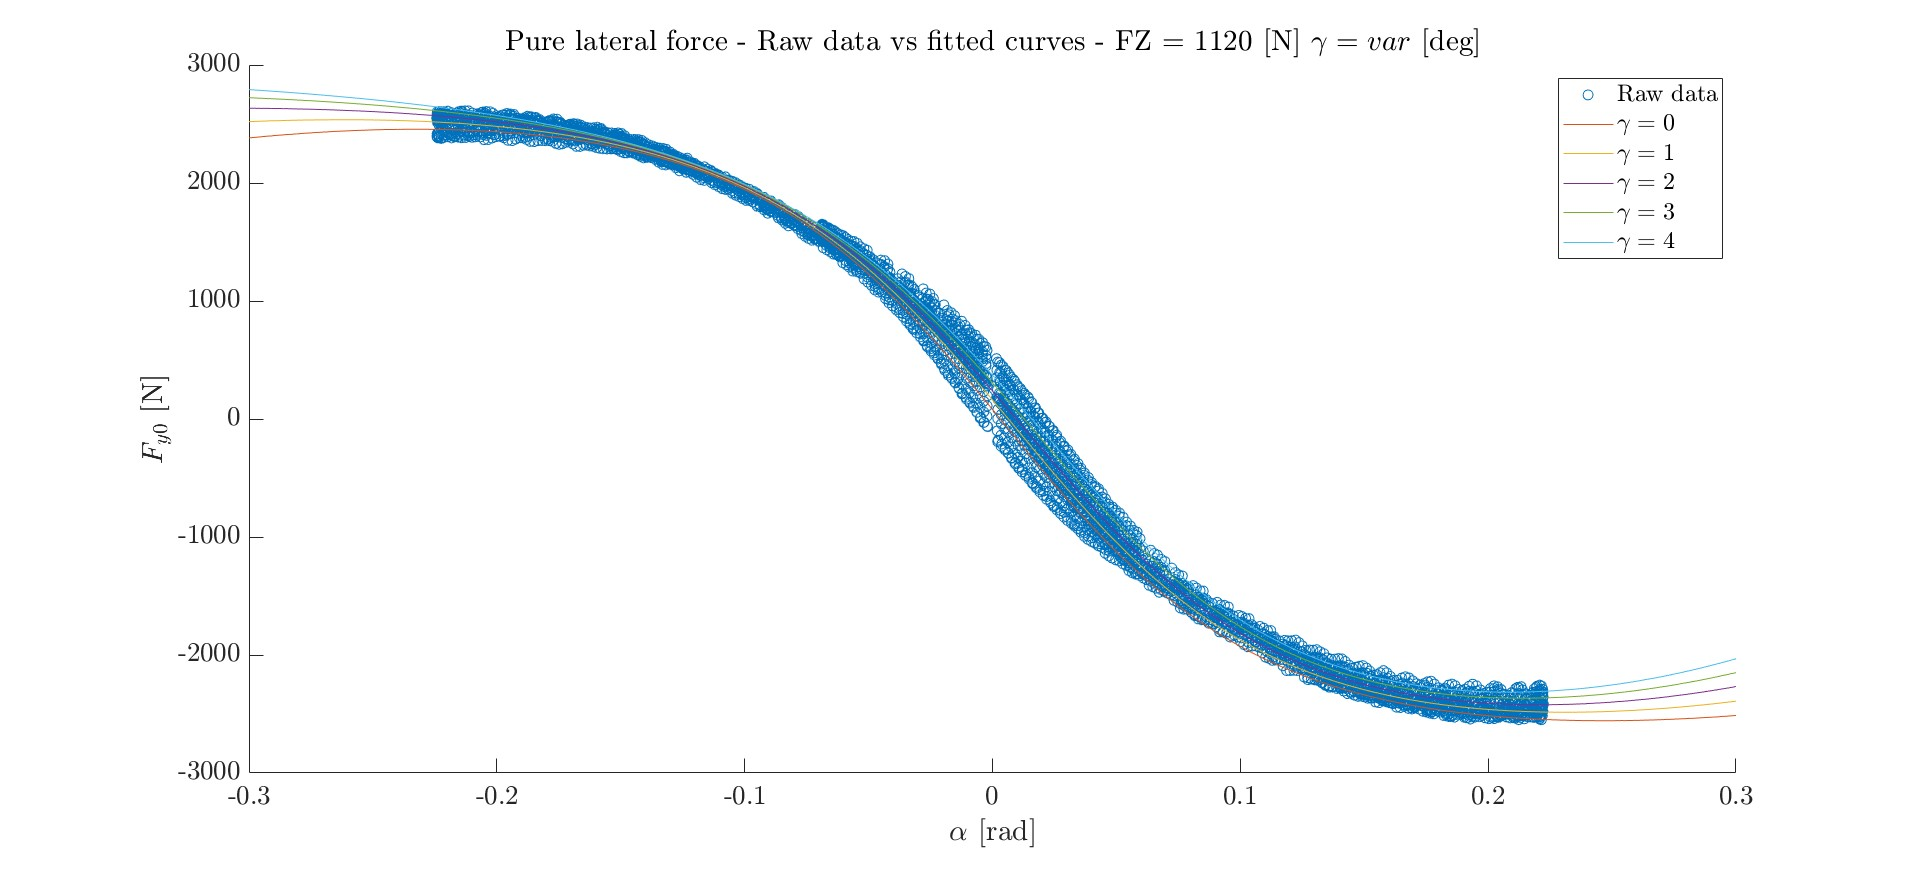
\includegraphics[width = 3.95in]{pure_lateral_3.jpg}}
                    
                    \label{fig:Fy0gam}
                \end{figure}
                
               

                \textbf{\textcolor{blue}{Obtained performance indexes}}: \\ $R^{2} = 99.84 \, \%$ and $RMSE = 73.49 \, $[N] .\\\\

            \item Fitting of coefficients depending both \textbf{on variable camber $\gamma$ and variable load $df_z$}
            
                \begin{table}[htbp]
                \begin{center}
                    \begin{tabular}{|l|l|}
                    \hline
                    Coefficients       & $pV_{y_4}$    \\
                    \hline
                    $P_0$ - initial guess & 0 \\ \hline
                    lb - lower bound   & -  \\ \hline
                    ub - upper bound   & -   \\ \hline
                    Fitted value       & 4.9444 \\ \hline
                    \end{tabular}
                    \end{center}
                \end{table}
                
                
                \begin{figure}[htbp]
                    \centerline{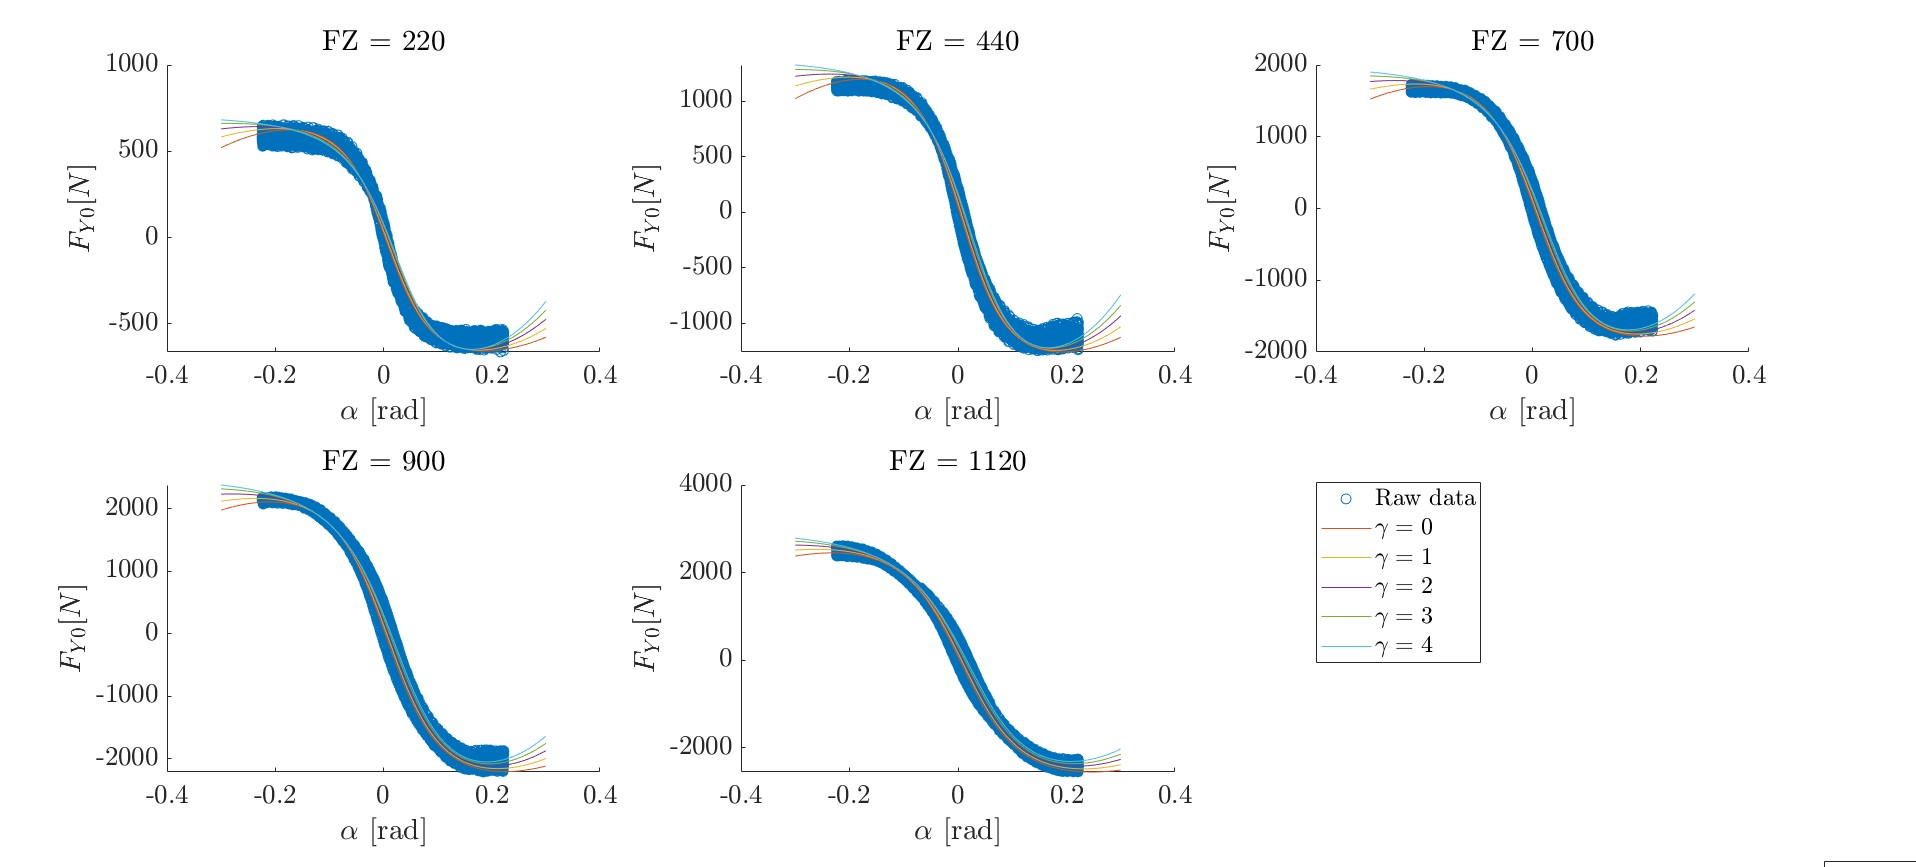
\includegraphics[width = 3.95in]{pure_lateral_4.jpg}}
                   
                    \label{fig:Fy0gam&dfz}
                \end{figure}

                \textbf{\textcolor{blue}{Obtained performance indexes}}: \\ $R^{2} = 99.62 \, \%$ and $RMSE = 77.57 $ \, [N] . \\\\
                \newpage
            The cornering stiffness $C_{F_\alpha}$ is shown below 
            \centerline{}
                \begin{figure}[h]
                    \centerline{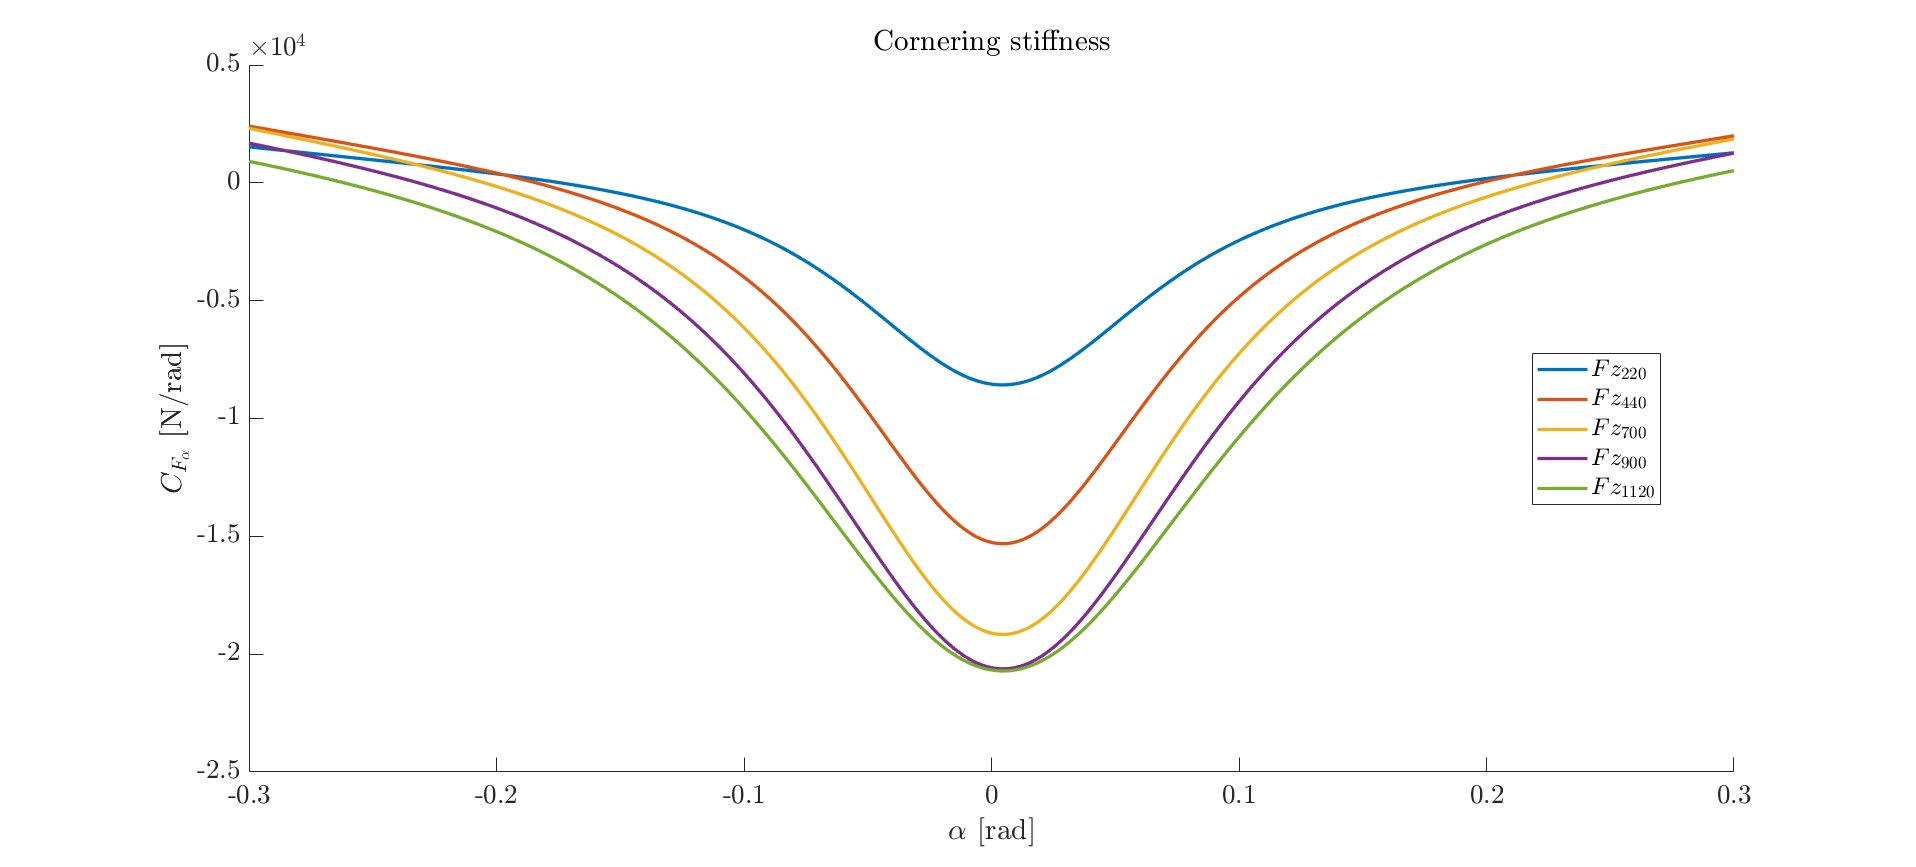
\includegraphics[width = 3.95in]{corneringK.jpg}}
                    
                    \label{fig:CornFy0}
                \end{figure}
            
        \end{itemize}
        
        
        \textit{\underline{COMMENTS}}: Differently from the fitting done for $F_{X0}$, the chosen nominal vertical load for the $F_{Y0}$'s coefficients is $1120 [N]$. This choice leads to more slack \texttt{fmincon} conditions and better fitted curves.
        It is of interest to note that the order of magnitude of the cornering stiffness peaks ranges from about 18 to 38 times the vertical wheel load. Pacejka\cite{pacejka} suggests that the usual range goes from about 6 to 30, with higher values for racing tyres, so the obtained range is compatible with the kind of racing tyre analysed.
        
        
    
        
        
    \subsection{\textbf{\underline{Combined Longitudinal Force}}}
        Fitting of the combined longitudinal force $F_{X}$ coefficients with the
        following step:
        \begin{itemize}
            \item Fitting of coefficients depending \textbf{on pure condition parameters with vertical nominal load $F_{z_0} = 220 \, [N]$ and zero camber angle $\gamma = 0 \, [deg] $} \\
 
                \begin{table}[htbp]
                \begin{center}
                    \begin{tabular}{|l|l|l|l|l|}
                    \hline
                    Coefficients       & $rB_{x_1}$ & $rB_{x_2}$ & $rC_{x_1}$  & $rH_{x_1}$   \\
                    \hline
                    $P_0$ - initial guess & 8.3 & 5 & 0.9 & 0 \\ \hline
                    lb - lower bound   & 7 & 0 & 0.5 & -100 \\ \hline
                    ub - upper bound   & 20 & 20 & 3 & 1 \\ \hline
                    Fitted value        & 14.6714 & 1.2440 & 1.0022& -19.3506 \\ \hline
                    \end{tabular}
                    \end{center}
                \end{table}
                
                \begin{figure}[htbp]
                    \centerline{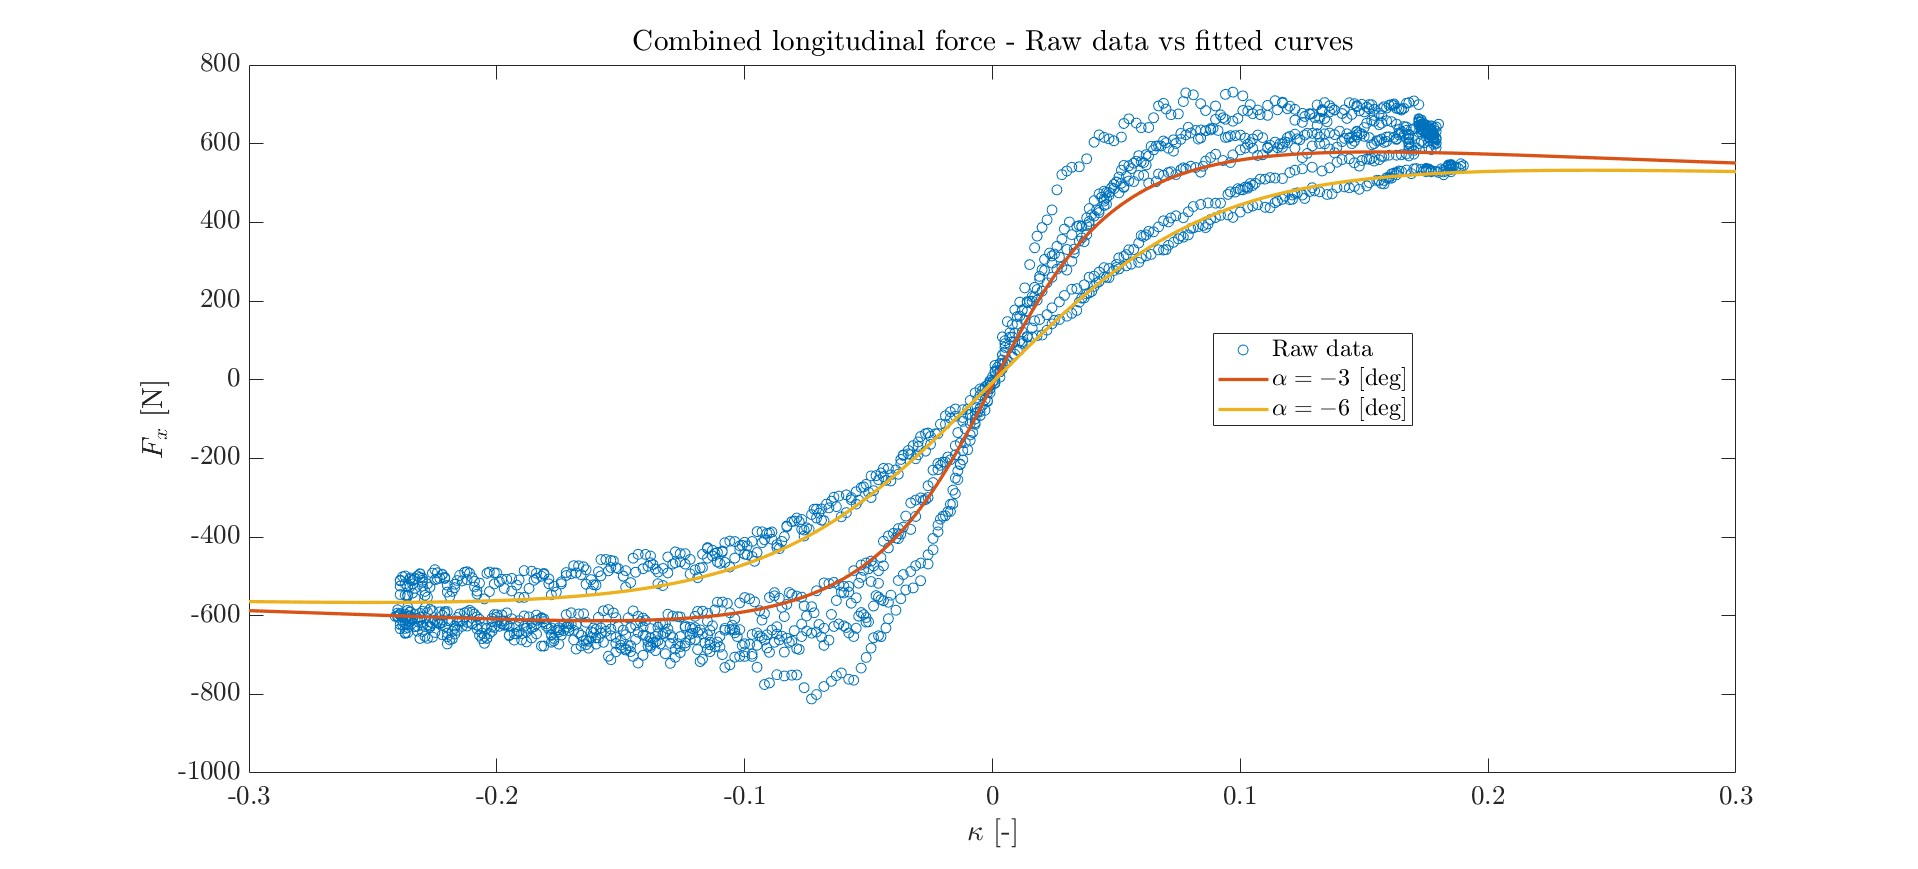
\includegraphics[width = 3.95in]{combined_longitudinal_1.jpg}}
                   
                    \label{fig:COMB_long_nom}
                \end{figure}
        \end{itemize}

        \textbf{\textcolor{blue}{Obtained performance indexes}}: \\ $R^{2} = 99.32 \, \%$ and $RMSE = 44.21 $ \, [N] . \\\\

        \newpage
        
        In the next figure it is shown the scaling factor $G_{x_a}$  as a function of the longitudinal slip $\kappa$
        
        \begin{figure}[htbp]
            \centerline{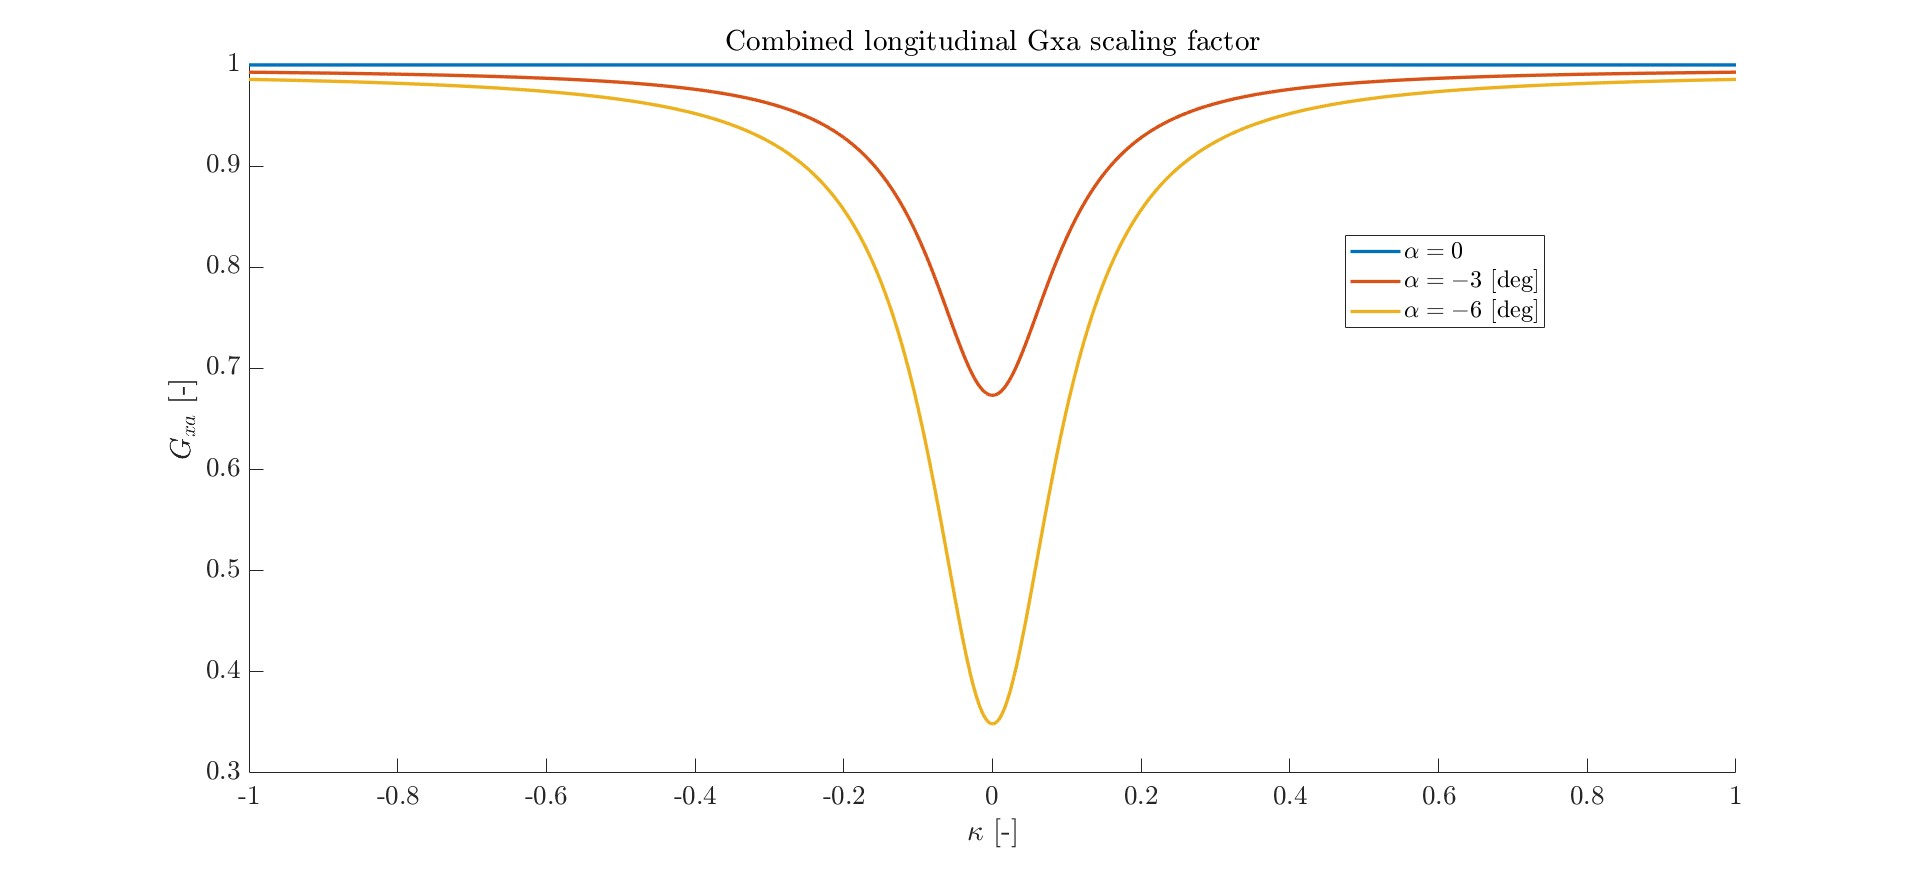
\includegraphics[width = 3.95in]{combined_longitudinal_2.jpg}}
            
            \label{fig:GXa}
        \end{figure}

        
    \subsection{\textbf{\underline{Combined Lateral Force}}}
        Fitting of the combined lateral force $F_{Y}$ coefficients with the following steps:
        \begin{itemize}
            \item Fitting of coefficients depending on \textbf{pure condition parameters with vertical nominal load $ F_{z_0} = 900 [N]$ and zero camber angle $\gamma = 0 \, [deg]$} \\
            
            \begin{table}[htbp]
                \begin{adjustbox}{width=\columnwidth,center}
                    \begin{tabular}{|l|l|l|l|l|l|l|l|l|l|}
                    \hline
                    Coefficients       & $rB_{y_1}$ & $rB_{y_2}$ & $rB_{y_3}$ & $rC_{y_1}$ & $rH_{y_1}$ & $rV_{y_1}$ & $rV_{y_4}$ & $rV_{y_5}$ & $rV_{y_6}$ \\
                    \hline
                    $P_0$ - initial guess & 4.9 & 2.2 & 0 & 1 & 0.1 & 0.1 & 30 & 0.5 & 10 \\ \hline
                    lb - lower bound   & -1000 & -1000 & -1000 & -1000 & -1000 & -1000 & -1000 & -1000 & -1000 \\ \hline
                    ub - upper bound   & 1000 & 1000 & 1000 & 1000 & 1000 & 1000 & 1000 & 1000 & 1000 \\ \hline
                    Fitted value  & 246.5833 & 973.0261 & -0.0750 & 0.9995 & 0.0453 & -4.0021 & 24.4909 & 0.0032 & 94.9144 \\ \hline
                    \end{tabular}
                \end{adjustbox}
            \end{table}          
                    
            \begin{figure}[htbp]
                \centerline{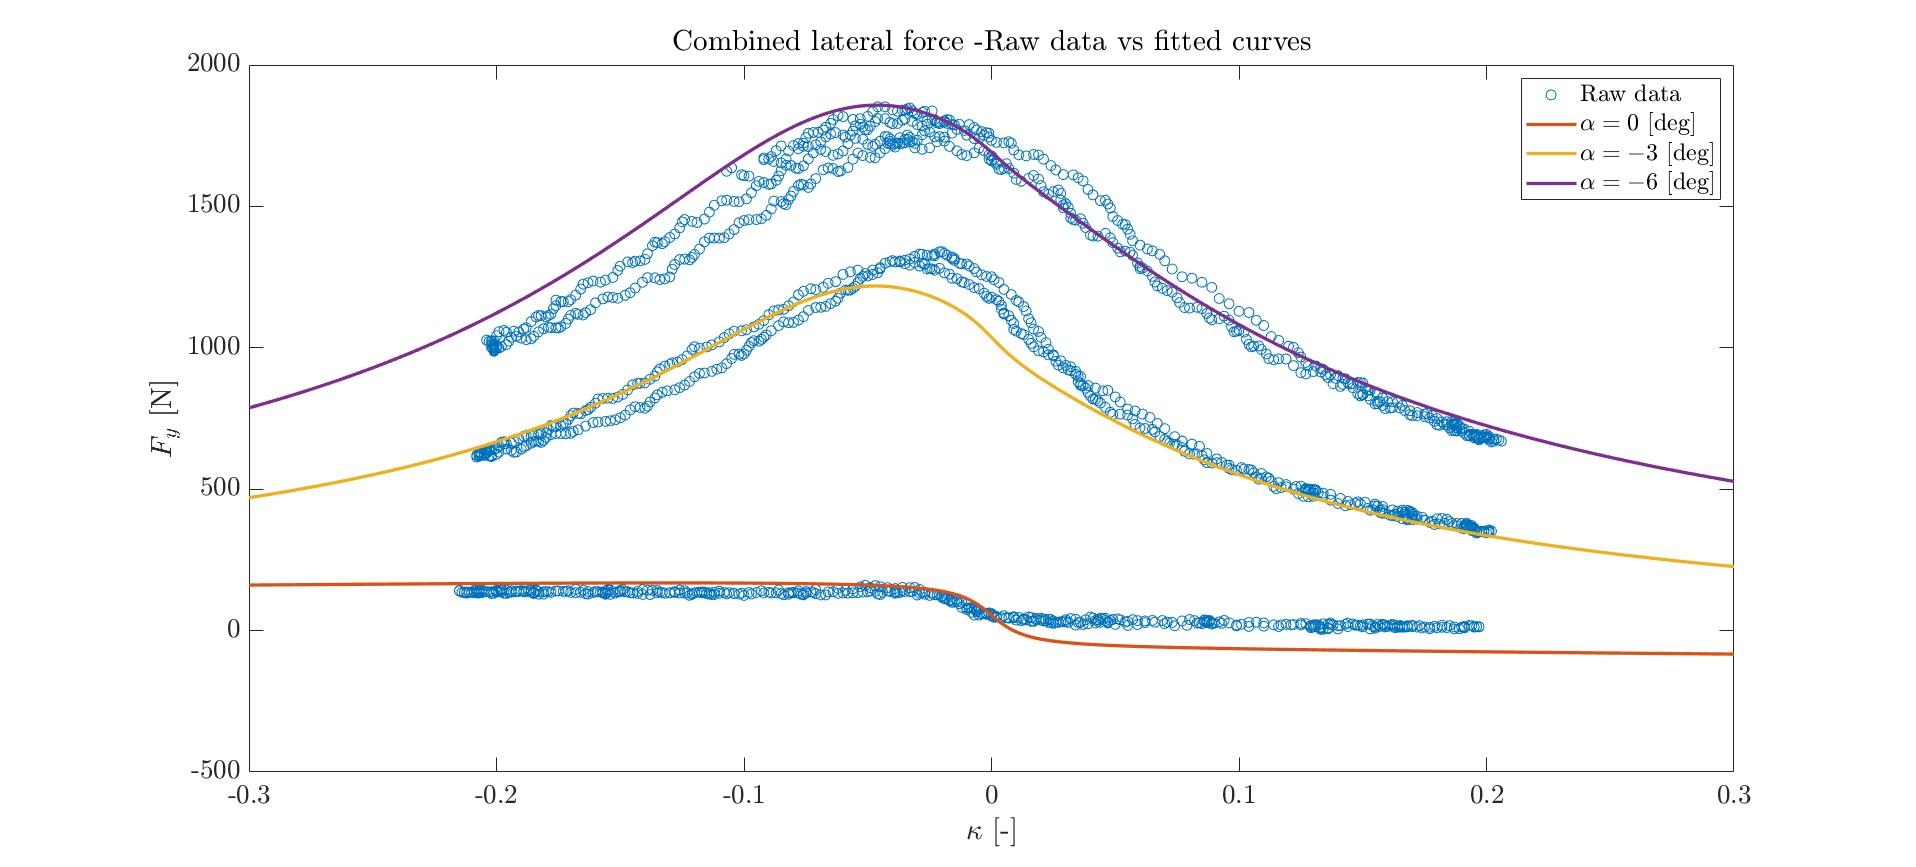
\includegraphics[width = 3.95in]{combined_lateral_1.jpg}}
                
                \label{fig:COMB_lat_nom}
            \end{figure}

            \textbf{\textcolor{blue}{Obtained performance indexes}}: \\ $R^{2} = 99.57 \, \%$ and $RMSE = 63.59 $ \, [N] . \\
        
            \item Fitting of coefficients depending on \underline{$df_z$} \textbf{load variation with zero camber angle $\gamma = 0$}\\
            \begin{table}[htbp]
                \begin{center}
                    \begin{tabular}{|l|l|}
                    \hline
                    Coefficients       & $rV_{y_2}$\\
                    \hline
                    $P_0$ - initial guess & 0 \\ \hline
                    lb - lower bound   & - \\ \hline
                    ub - upper bound   & - \\ \hline
                    Fitted value  & -9.8945 \\ \hline
                    \end{tabular}
                \end{center}
            \end{table} 
            \newpage
             \begin{figure}[!h]
                \centerline{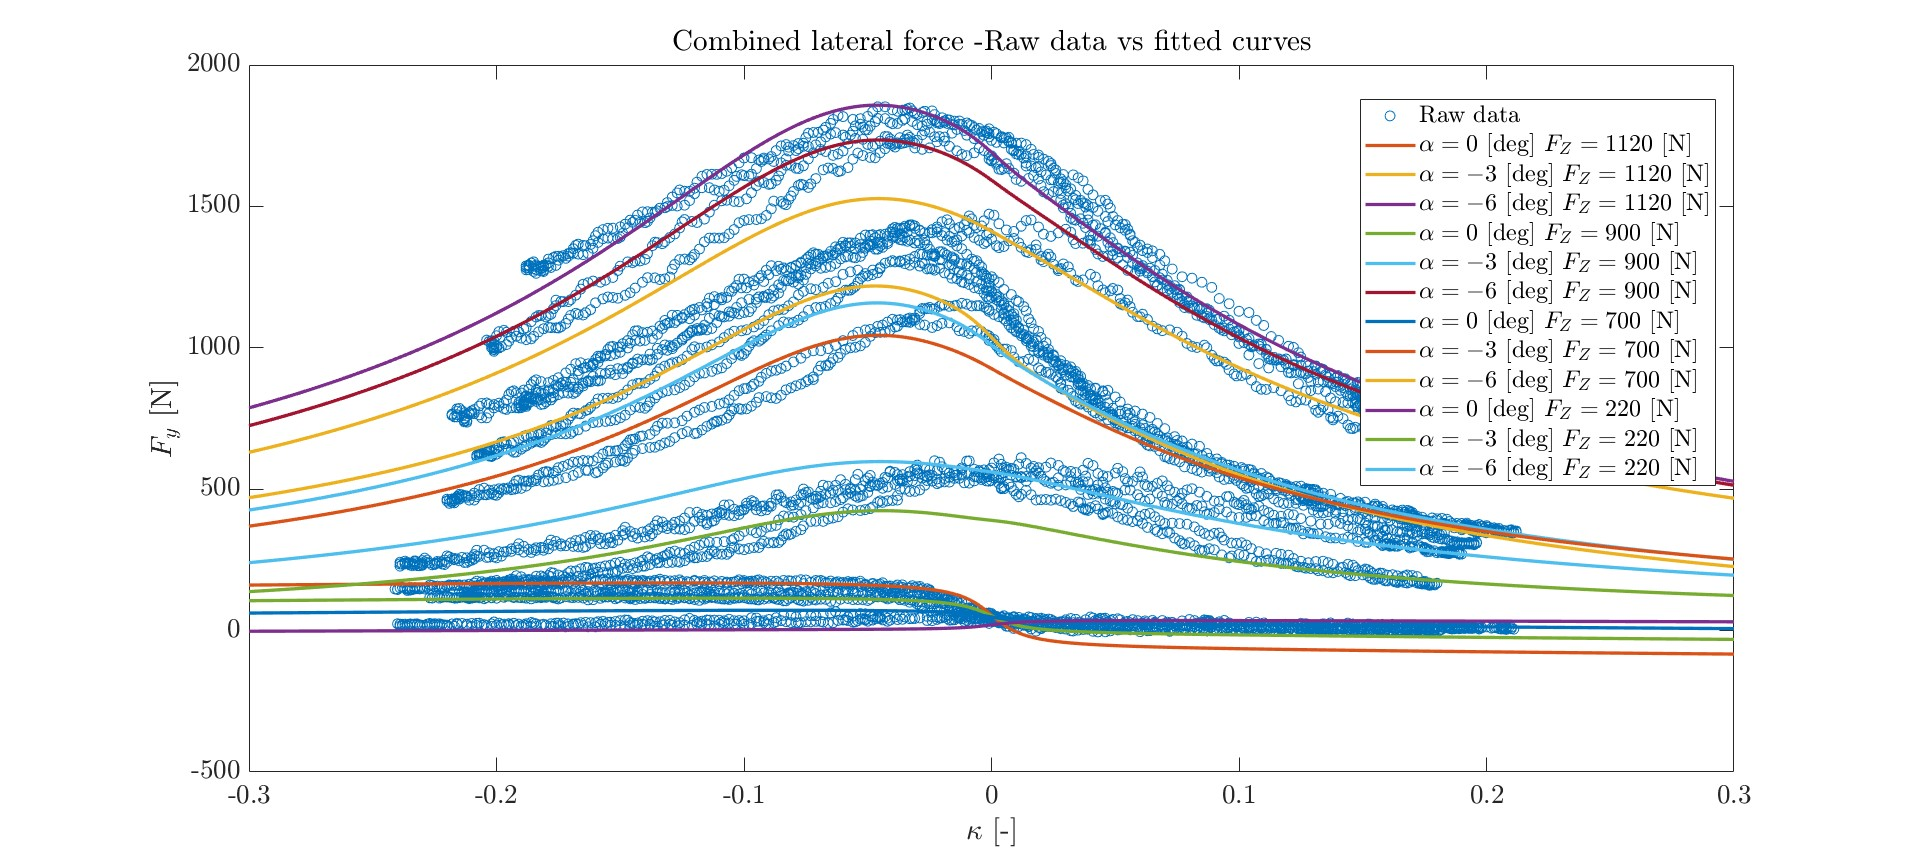
\includegraphics[width = 3.95in]{combined_lateral_3.jpg}}
                
                \label{fig:COMB_lat_dfz}
            \end{figure}
            
           

            \textbf{\textcolor{blue}{Obtained performance indexes}}: \\ $R^{2} = 99.19 \, \%$ and $RMSE = 67.91 $ \, [N] . \\

            
            
            \item Fitting of coefficients depending \textbf{on variable camber conditions and nominal vertical load $F_{z_0} = 900 $ \, [N]}\\
            
            \begin{table}[!h]
                \begin{center}
                    \begin{tabular}{|l|l|}
                    \hline
                    Coefficients       & $rV_{y_3}$\\
                    \hline
                    $P_0$ - initial guess & 0 \\ \hline
                    lb - lower bound   & - \\ \hline
                    ub - upper bound   & - \\ \hline
                    Fitted value  & -31.6715 \\ \hline
                    \end{tabular}
                \end{center}
            \end{table} 
            
        
         \begin{figure}[!h]
                \centerline{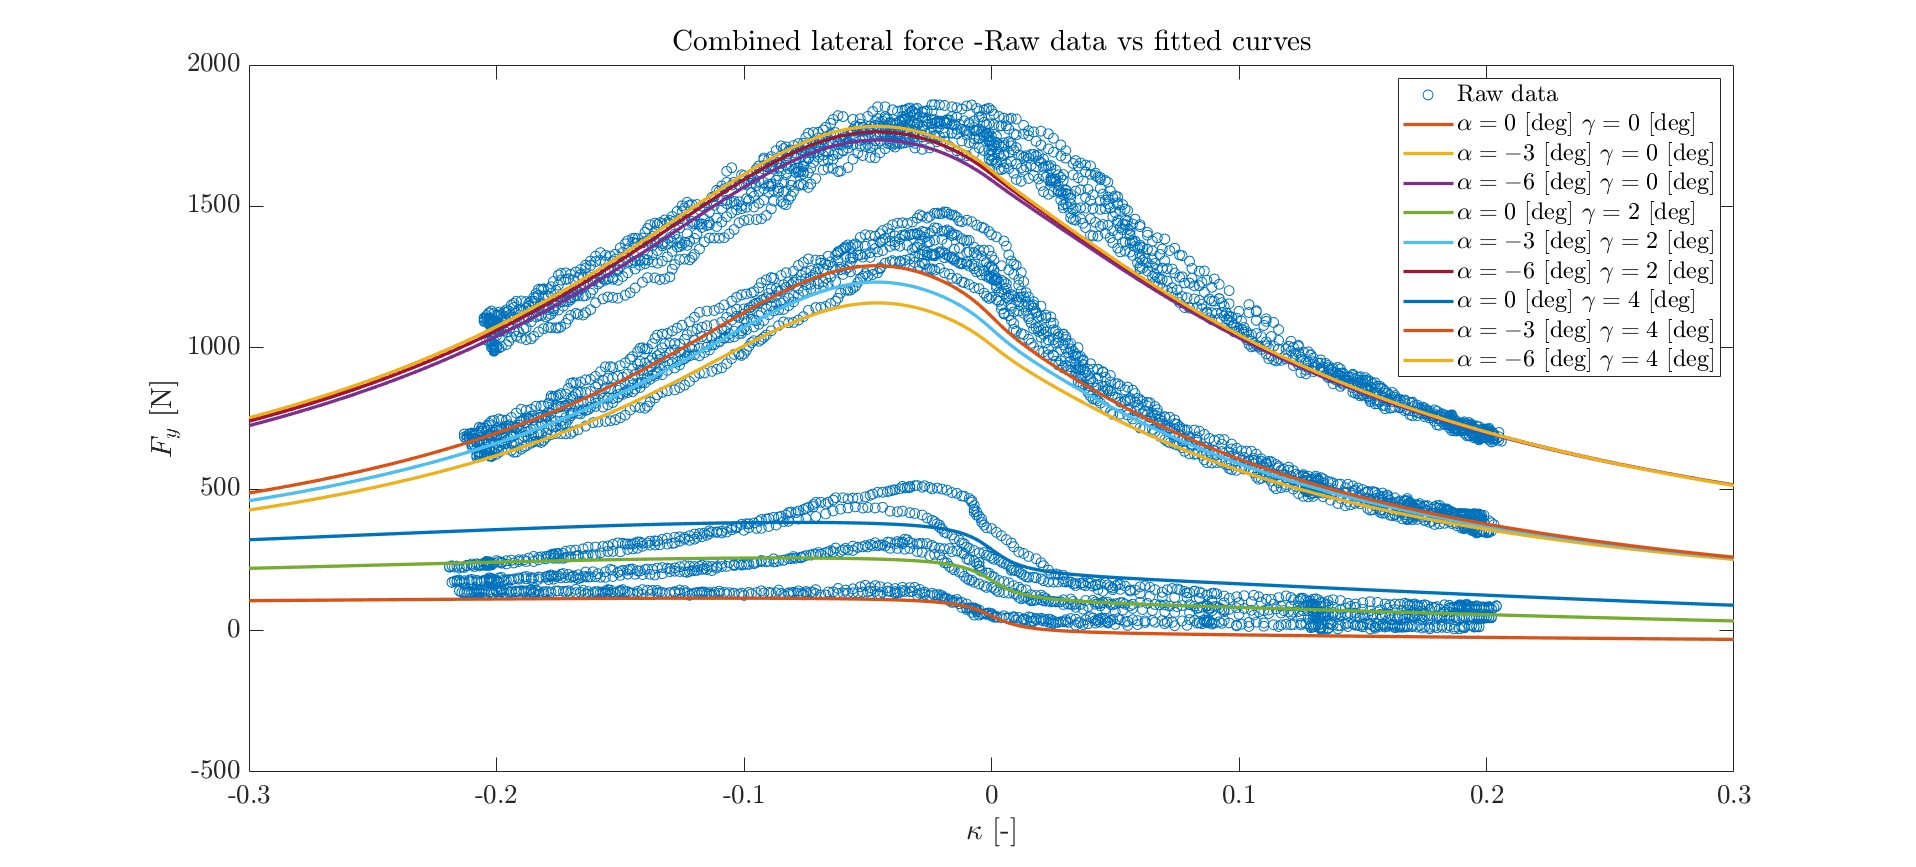
\includegraphics[width = 3.95in]{combined_lateral_4.jpg}}
                
                \label{fig:COMB_lat_varGamma}
            \end{figure}
            

        \textbf{\textcolor{blue}{Obtained performance indexes}}: \\ $R^{2} = 97.50 \, \%$ and $RMSE = 149.69 $ \, [N] . \\\\

        In the next figure it is shown the scaling factor $G_{y_\kappa}$  for the combined lateral force $F_y$
        
        \begin{figure}[!h]
            \centerline{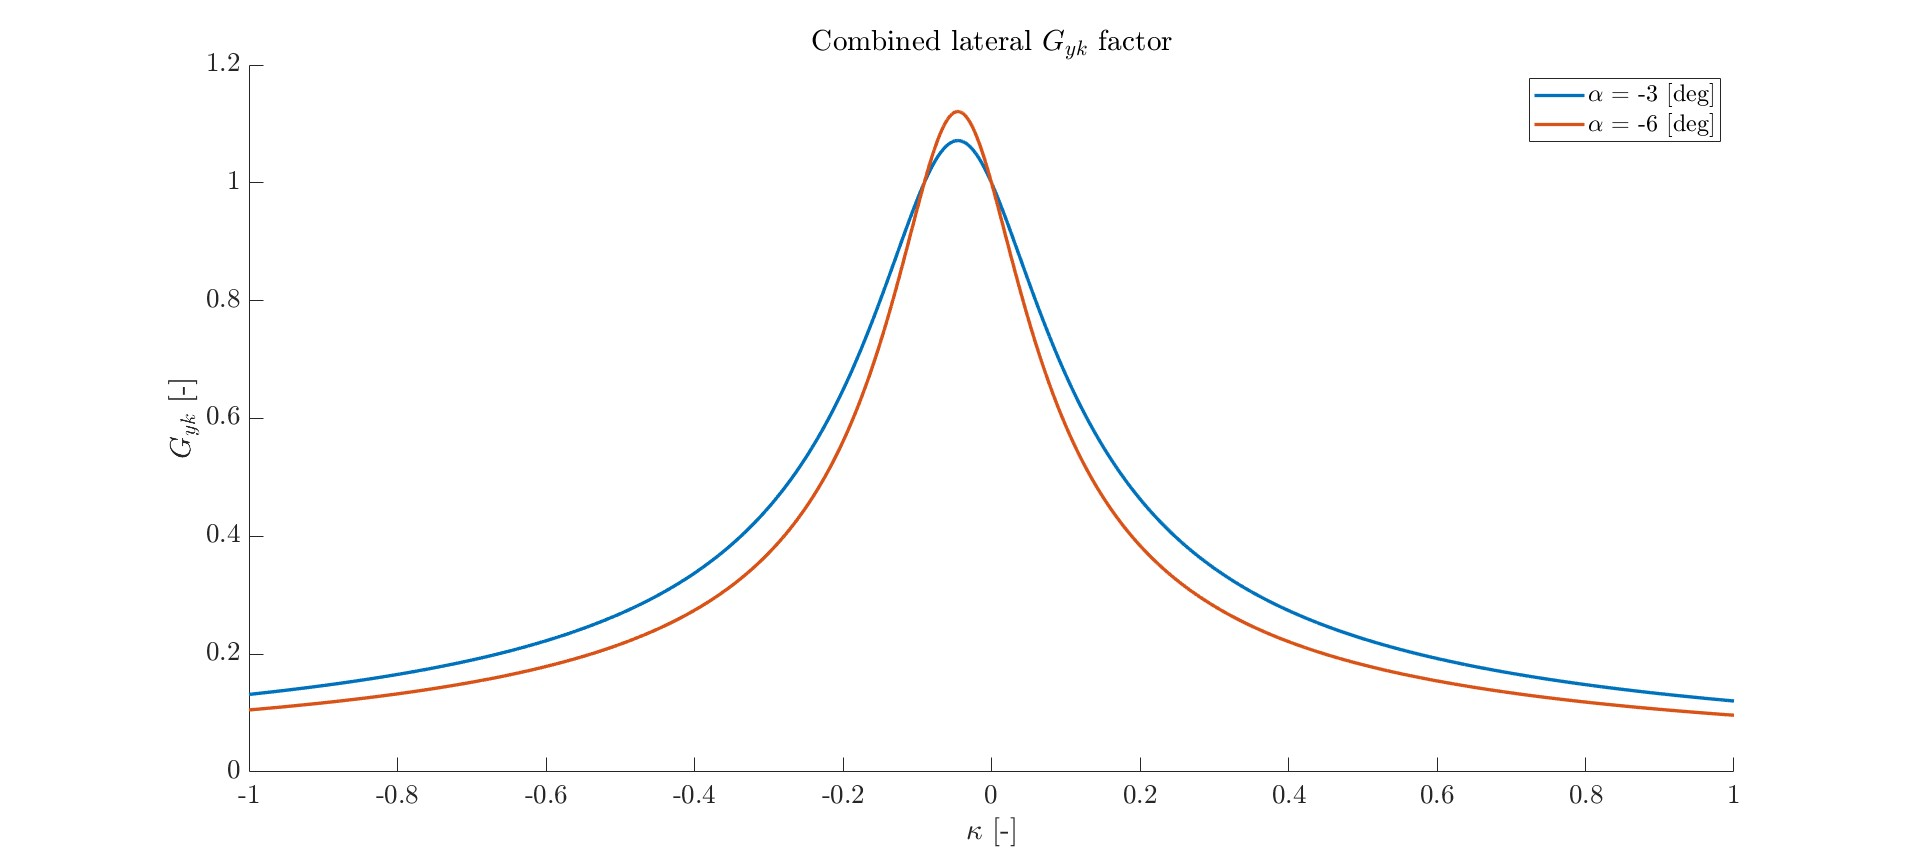
\includegraphics[width = 3.95in]{combined_lateral_2.jpg}}
            
            \label{fig:Gyk}
        \end{figure}
    \end{itemize}
    
    \textit{\underline{COMMENTS}}: Combined behaviour fittings were the hardest to achieve, the overall result may be inaccurate for some load/camber configurations. A finer tuning of the coefficients may solve the problem. Similarly to $F_{Y_0}$ fitting, the $F_{Z_0}$ nominal load has been changed to $900$ [N] in order to get better results.
    \newpage
    \subsection{\textbf{\underline{Pure Self-Aligning Moment}}}
    Fitting of the Self-Aligning Moment $M_{z_0}$ coefficients with the following steps:
                
        \begin{itemize}
            \item Fitting of coefficients with \textbf{pure conditions:  vertical nominal load $F_{z_0} = 1120 \, [N]$ and zero camber angle $\gamma = 0 \, [deg]$}  \\
        
                \begin{table}[htbp]
                    \begin{adjustbox}{width=\columnwidth,center}
                        \begin{tabular}{|l|l|l|l|l|l|l|l|l|l|}  
                            \hline
                            Coefficients & $qH_{z_1}$ & $qB_{z_1}$ & $qC_{z_1}$ & $qD_{z_1}$ & $qE_{z_1}$ & $qE_{z_4}$ &
                            $qB_{z_9}$ & $qB_{z_{10}}$ & $qD_{z_6}$ \\
                            \hline
                            $P_0$ - initial guess & 0.1 & 0.1 & 0.1 & 0.1 & 0.1 & 0.1 & 0.1 & 0.1 & 0.1 \\ \hline
                            lb - lower bound   & - & - & - & - & - & - & - & - & - \\ 
                            \hline
                            ub - upper bound   & - & - & - & - & - & - & - & - & - \\ 
                            \hline
                            Fitted value & -0.0132 & 6.2738 & 1.7473 & 0.2400 & 0.4249 & -0.1461 & 0.2299 & -0.5407 & -0.0045 \\
                            \hline
                        \end{tabular}
                    \end{adjustbox}
                \end{table}
            
                \begin{figure}[htbp]
                    \centerline{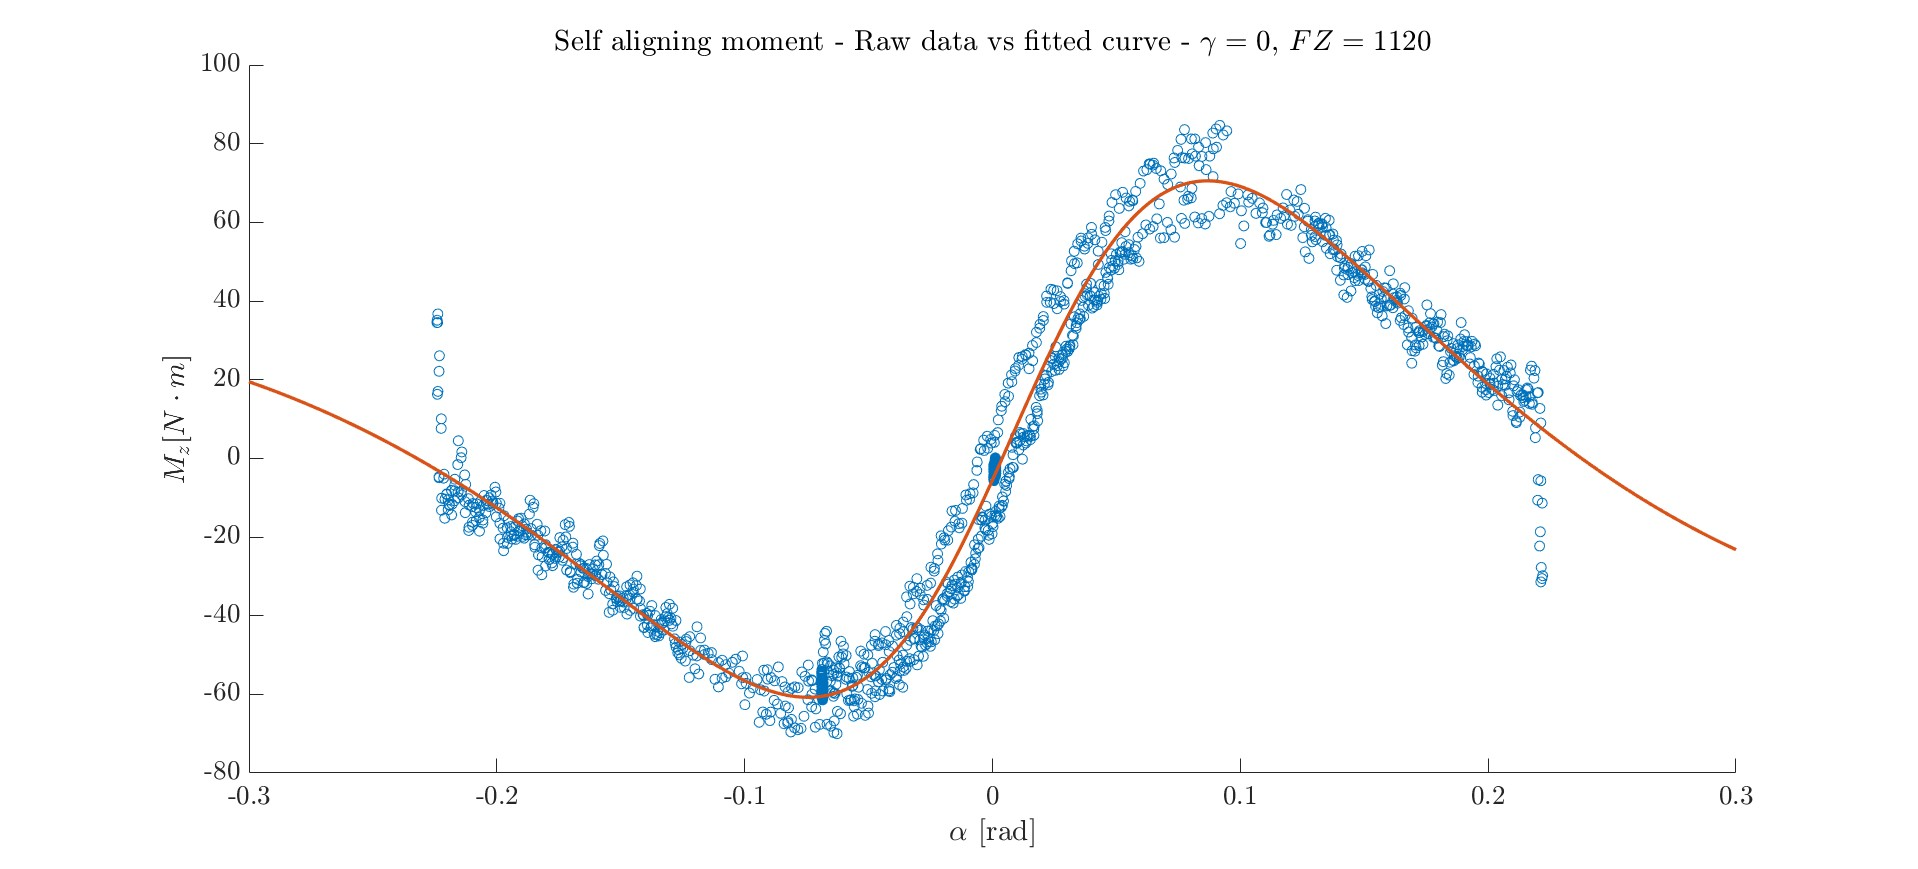
\includegraphics[width = 3.95in]{moment_1.jpg}}
                    \label{fig:MZ_nom}
                \end{figure}

                \textbf{\textcolor{blue}{Obtained performance indexes}}: \\ $R^{2} = 97.26 \, \%$ and $RMSE = 6.38 $ \, [N$\cdot$m] . \\\\
                
            \item Fitting of coefficients depending on \textbf{\underline{$df_z$} load variation with zero camber angle $\gamma = 0$}
                \begin{table}[htbp]
                    \begin{adjustbox}{width=\columnwidth,center}
                        \begin{tabular}{|l|l|l|l|l|l|l|l|}  
                            \hline
                            Coefficients & $qH_{z_2}$ & $qB_{z_2}$ & $qB_{z_3}$ & $qD_{z_2}$ & $qE_{z_2}$ & $qE_{z_3}$ & $qD_{z_7}$ \\
                            \hline
                            $P_0$ - initial guess & 0.1 & 0.1 & 0.1 & 0.1 & 0.1 & 0.1 &\\ \hline
                            lb - lower bound   & - & - & - & - & - & - & -\\ 
                            \hline
                            ub - upper bound   & - & - & - & - & - & - &\\ 
                            \hline
                            Fitted value & -0.0024 & -0.8874 & -0.9187 & -0.0254 & -0.3624 & -1.2557 & -0.0156 \\
                            \hline
                        \end{tabular}
                    \end{adjustbox}
                \end{table}
            
                \begin{figure}[!h]
                    \centerline{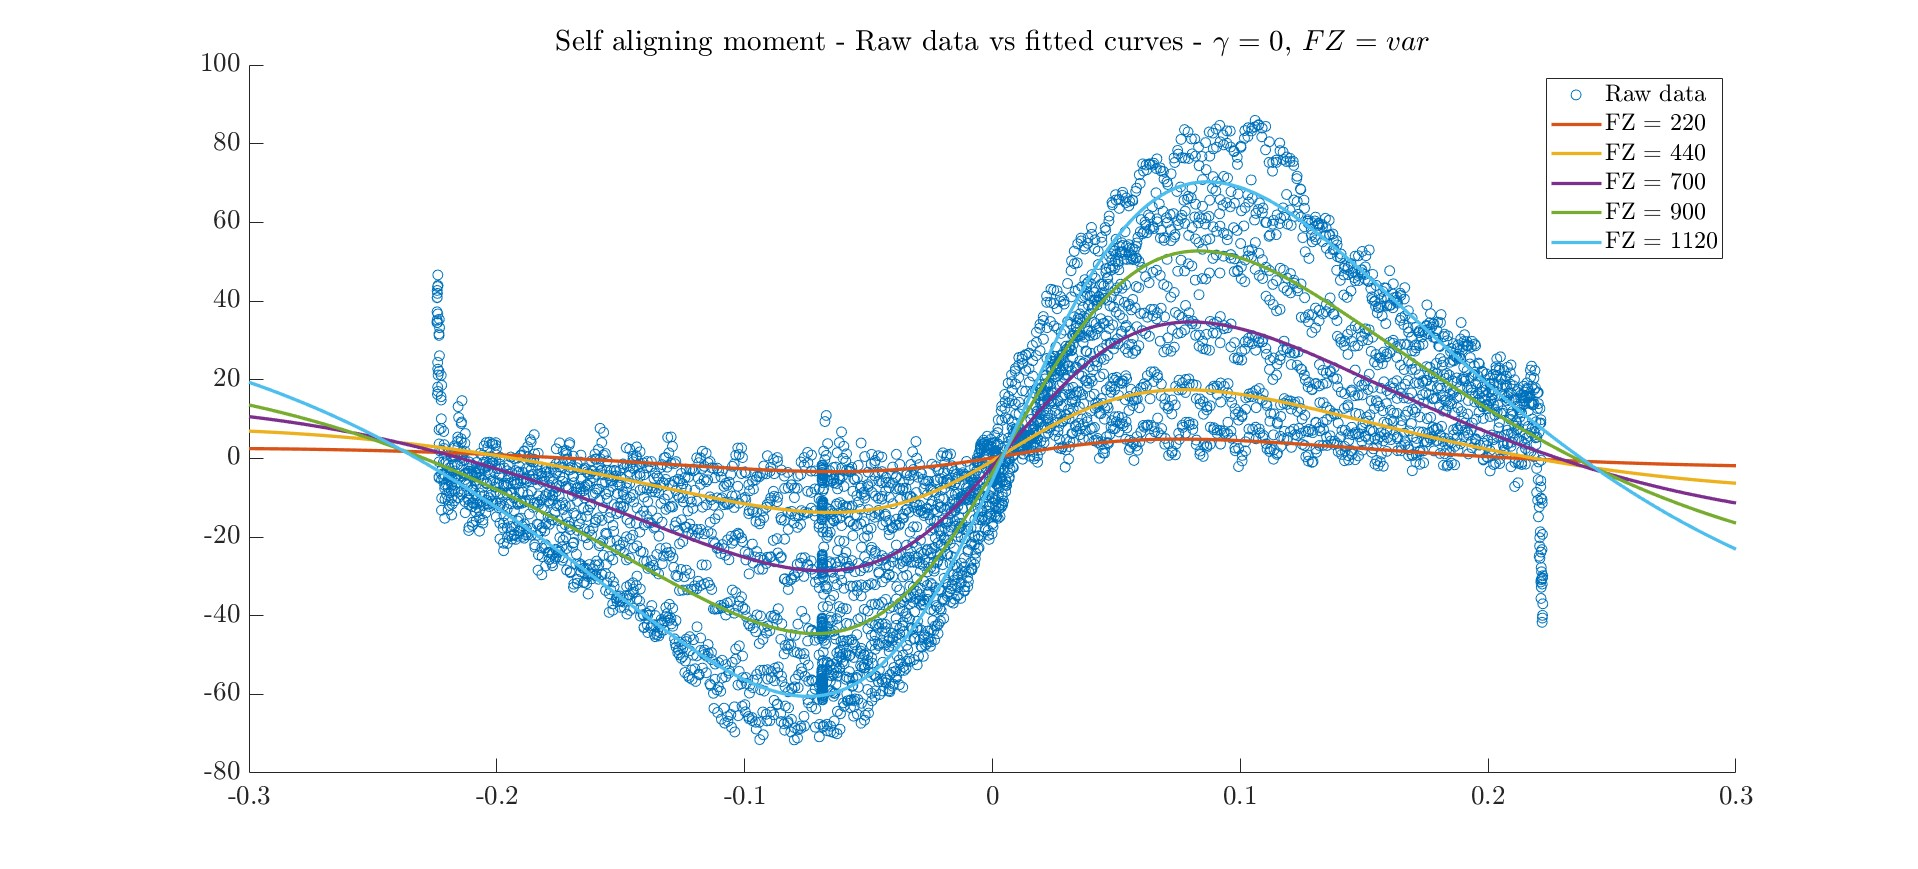
\includegraphics[width = 3.95in]{moment_2.jpg}}
                    
                    \label{fig:MZ_dfz}
                \end{figure}
                
                \textbf{\textcolor{blue}{Obtained performance indexes}}: \\ $R^{2} = 96.82 \, \%$ and $RMSE = 5.3459 $ \, [N$\cdot$m] . \\\\
                
            \newpage
            
            \item Fitting of coefficients depending \textbf{on variable camber $\gamma$ with nominal vertical load $F_{z_0} = 1120 $ \, [N]}
                \begin{table}[htbp]
                    \begin{adjustbox}{width=\columnwidth,center}
                        \begin{tabular}{|l|l|l|l|l|l|l|l|}  
                            \hline
                            Coefficients & $qH_{z_3}$ & $qB_{z_4}$ & $qB_{z_5}$ & $qD_{z_3}$ & $qD_{z_4}$ & $qE_{z_5}$ & $qD_{z_8}$  \\
                            \hline
                            $P_0$ - initial guess & 0.1 & 0.1 & 0.1 & 0.1 & 0.1 & 0.1 & 0.1\\ \hline
                            lb - lower bound   & - & - & - & - & - & - & -\\ 
                            \hline
                            ub - upper bound   & - & - & - & - & - & - & -\\ 
                            \hline
                            Fitted value & 0.7460 & -7.3893 & 6.6463 & -1.0072 & 4.7283 & -2.5673 & 1.7837  \\
                            \hline
                        \end{tabular}
                    \end{adjustbox}
                \end{table}

                \begin{figure}[htbp]
                    \centerline{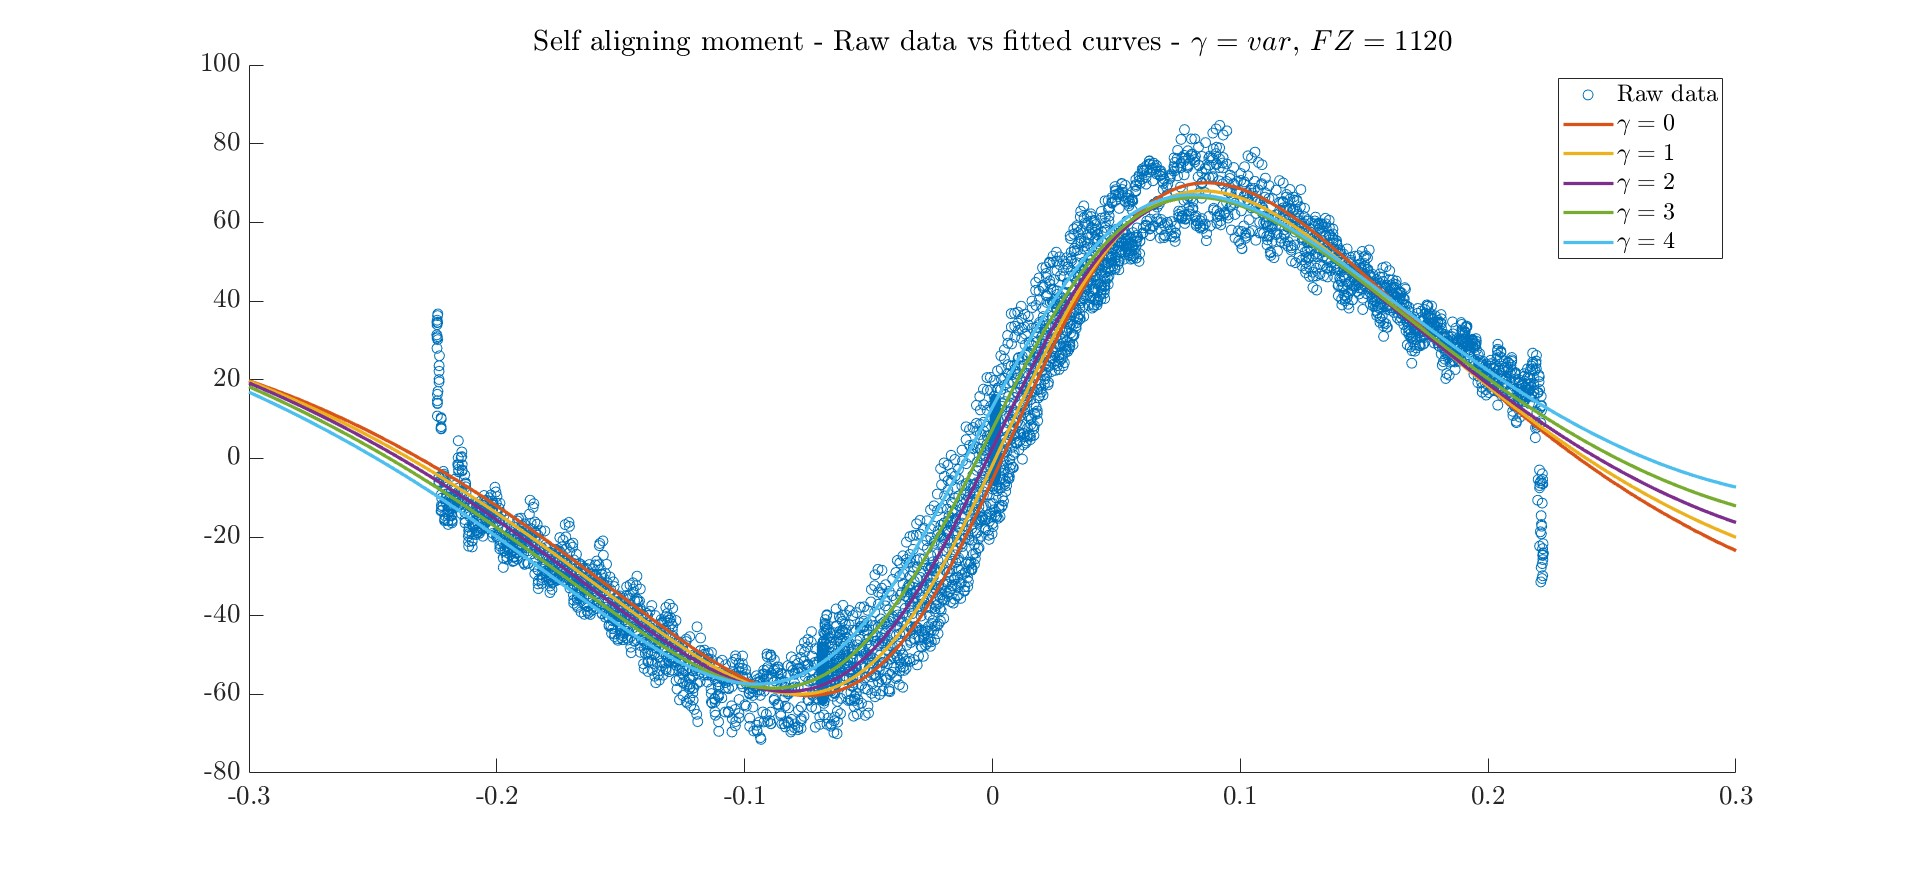
\includegraphics[width = 3.95in]{moment_3.jpg}}
                    \caption{\textbf{Variable camber conditions: plots of raw data and fitting }}
                    \label{fig:MZ_camber}
                \end{figure}

                
                \textbf{\textcolor{blue}{Obtained performance indexes}}: \\ $R^{2} = 97.40 \, \%$ and $RMSE = 6.5335 $ \, [N$\cdot$m] . \\\\

            
                
            \item Fitting of coefficients depending on both \textbf{variable camber $\gamma$ and variable load $df_z$}
            
                \begin{table}[htbp]
                    \begin{center}
                    \begin{tabular}{|l|l|l|}  
                        \hline
                        Coefficients & $qD_{z_9}$ & $qH_{z_4}$ \\
                        \hline
                        $P_0$ - initial guess & 1 & 0.5\\ \hline
                        lb - lower bound   & 0.9 & 0.4 \\ 
                        \hline
                        ub - upper bound   & 1.1 & 0.6 \\ 
                        \hline
                        Fitted value & 0.9000 & 0.5168 \\
                        \hline
                    \end{tabular}
                    \end{center}
                \end{table}
                
            
                \begin{figure}[htbp]
                    \centerline{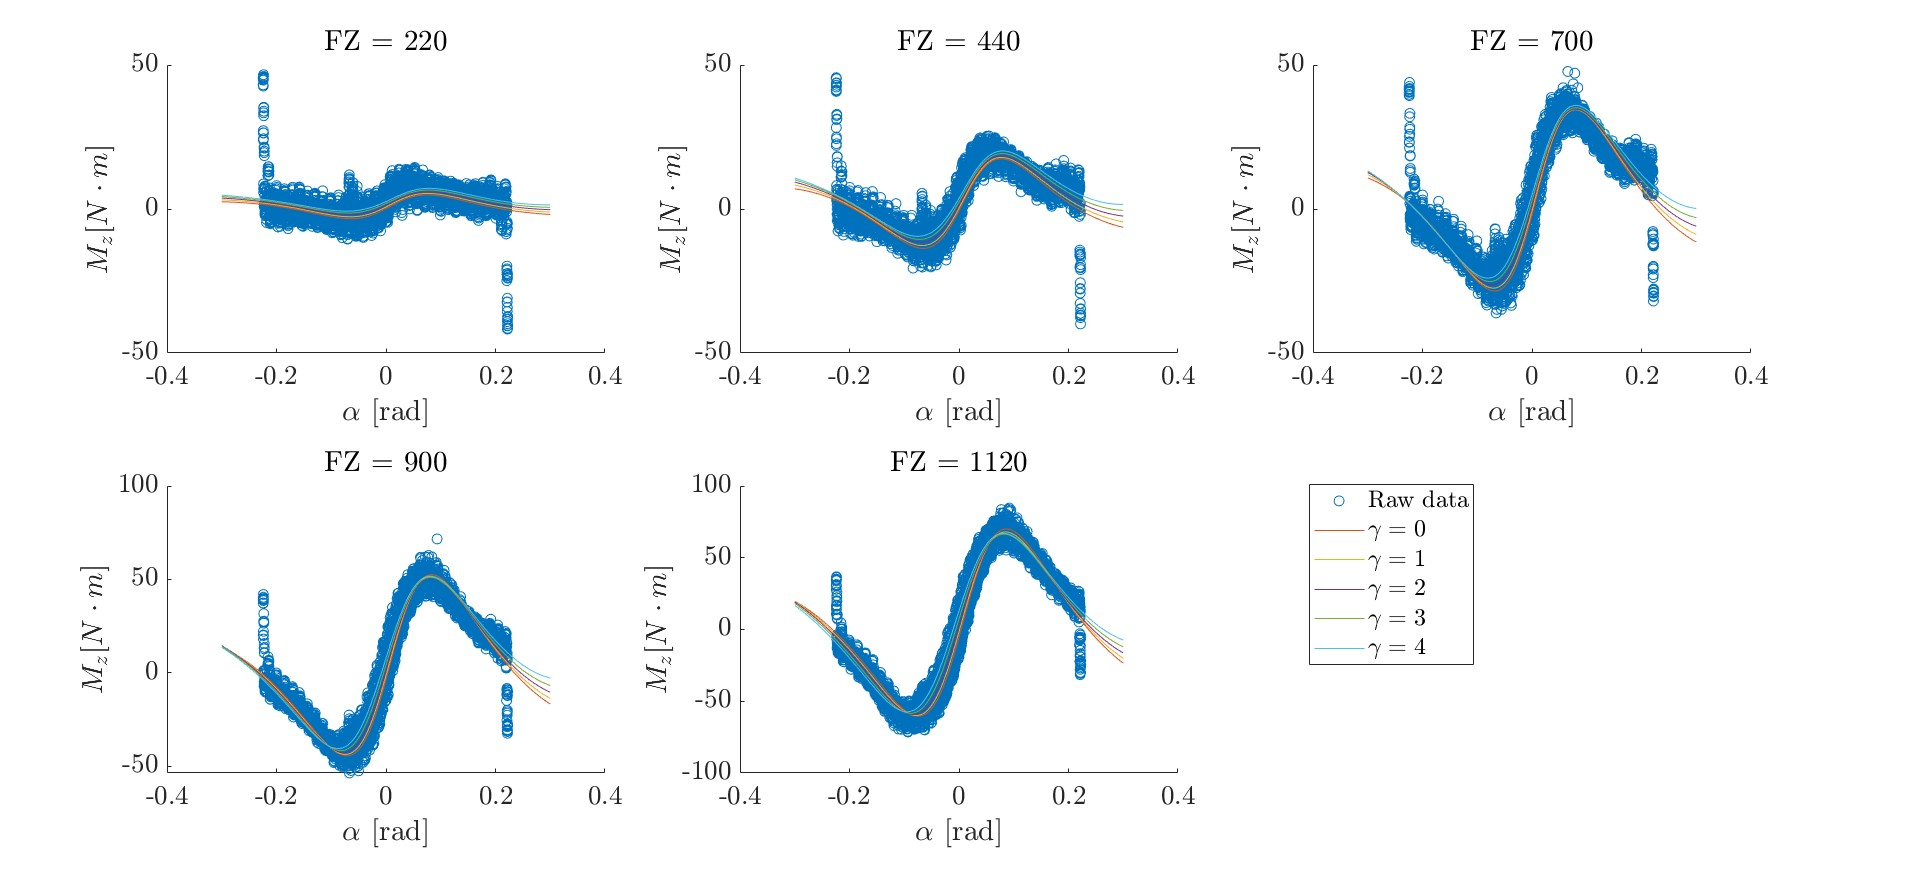
\includegraphics[width = 3.95in]{moment_4.jpg}}
                    
                    \label{fig:MZ_camber_dfz}
                \end{figure}
            \end{itemize}
            
            \textbf{\textcolor{blue}{Obtained performance indexes}}: \\ $R^{2} = 96.17 \, \%$ and $RMSE = 5.2640 $ \, [N$\cdot$m] . \\\\

            \textit{\underline{COMMENTS}}: Using $F_{Z0} = 1120\,[N]$, the obtained curves fit well the actual data. The latter two coefficients needed stricter bounds in order to fit better the curves.

        \newpage
        
    \begin{thebibliography}{00}
        \bibitem{b1} Biral Francesco, Semi empirical tyre models; Magic Formula 96, Trento: Italy, 2023, pp. 34 -- 45.
        \bibitem{pacejka} Hans B. Pacejka, Tyre and Vehicle Dynamics, Second edition, Oxford: Butterworth-Heinemann, 2006
        \bibitem{b3} Delfttyre TNO, MF-Tyre/MF-Swift 6.2
        Help Manual, Document revision: 10/17/2013. The Netherlands, 2013. \\\\
        
    \end{thebibliography}
\end{document}
